%  LaTeX support: latex@mdpi.com 
%  For support, please attach all files needed for compiling as well as the log file, and specify your operating system, LaTeX version, and LaTeX editor.

%=================================================================
\documentclass[journal,article,submit,pdftex,moreauthors]{Definitions/mdpi} 

%--------------------
% Class Options:
%--------------------
%----------
% journal
%----------
% Choose between the following MDPI journals:
% acoustics, actuators, addictions, admsci, adolescents, aerobiology, aerospace, agriculture, agriengineering, agrochemicals, agronomy, ai, air, algorithms, allergies, alloys, analytica, analytics, anatomia, animals, antibiotics, antibodies, antioxidants, applbiosci, appliedchem, appliedmath, applmech, applmicrobiol, applnano, applsci, aquacj, architecture, arm, arthropoda, arts, asc, asi, astronomy, atmosphere, atoms, audiolres, automation, axioms, bacteria, batteries, bdcc, behavsci, beverages, biochem, bioengineering, biologics, biology, biomass, biomechanics, biomed, biomedicines, biomedinformatics, biomimetics, biomolecules, biophysica, biosensors, biotech, birds, bloods, blsf, brainsci, breath, buildings, businesses, cancers, carbon, cardiogenetics, catalysts, cells, ceramics, challenges, chemengineering, chemistry, chemosensors, chemproc, children, chips, cimb, civileng, cleantechnol, climate, clinpract, clockssleep, cmd, coasts, coatings, colloids, colorants, commodities, compounds, computation, computers, condensedmatter, conservation, constrmater, cosmetics, covid, crops, cryptography, crystals, csmf, ctn, curroncol, cyber, dairy, data, ddc, dentistry, dermato, dermatopathology, designs, devices, diabetology, diagnostics, dietetics, digital, disabilities, diseases, diversity, dna, drones, dynamics, earth, ebj, ecologies, econometrics, economies, education, ejihpe, electricity, electrochem, electronicmat, electronics, encyclopedia, endocrines, energies, eng, engproc, entomology, entropy, environments, environsciproc, epidemiologia, epigenomes, est, fermentation, fibers, fintech, fire, fishes, fluids, foods, forecasting, forensicsci, forests, foundations, fractalfract, fuels, future, futureinternet, futurepharmacol, futurephys, futuretransp, galaxies, games, gases, gastroent, gastrointestdisord, gels, genealogy, genes, geographies, geohazards, geomatics, geosciences, geotechnics, geriatrics, grasses, gucdd, hazardousmatters, healthcare, hearts, hemato, hematolrep, heritage, higheredu, highthroughput, histories, horticulturae, hospitals, humanities, humans, hydrobiology, hydrogen, hydrology, hygiene, idr, ijerph, ijfs, ijgi, ijms, ijns, ijpb, ijtm, ijtpp, ime, immuno, informatics, information, infrastructures, inorganics, insects, instruments, inventions, iot, j, jal, jcdd, jcm, jcp, jcs, jcto, jdb, jeta, jfb, jfmk, jimaging, jintelligence, jlpea, jmmp, jmp, jmse, jne, jnt, jof, joitmc, jor, journalmedia, jox, jpm, jrfm, jsan, jtaer, jvd, jzbg, kidneydial, kinasesphosphatases, knowledge, land, languages, laws, life, liquids, literature, livers, logics, logistics, lubricants, lymphatics, machines, macromol, magnetism, magnetochemistry, make, marinedrugs, materials, materproc, mathematics, mca, measurements, medicina, medicines, medsci, membranes, merits, metabolites, metals, meteorology, methane, metrology, micro, microarrays, microbiolres, micromachines, microorganisms, microplastics, minerals, mining, modelling, molbank, molecules, mps, msf, mti, muscles, nanoenergyadv, nanomanufacturing,\gdef\@continuouspages{yes}} nanomaterials, ncrna, ndt, network, neuroglia, neurolint, neurosci, nitrogen, notspecified, %%nri, nursrep, nutraceuticals, nutrients, obesities, oceans, ohbm, onco, %oncopathology, optics, oral, organics, organoids, osteology, oxygen, parasites, parasitologia, particles, pathogens, pathophysiology, pediatrrep, pharmaceuticals, pharmaceutics, pharmacoepidemiology,\gdef\@ISSN{2813-0618}\gdef\@continuous pharmacy, philosophies, photochem, photonics, phycology, physchem, physics, physiologia, plants, plasma, platforms, pollutants, polymers, polysaccharides, poultry, powders, preprints, proceedings, processes, prosthesis, proteomes, psf, psych, psychiatryint, psychoactives, publications, quantumrep, quaternary, qubs, radiation, reactions, receptors, recycling, regeneration, religions, remotesensing, reports, reprodmed, resources, rheumato, risks, robotics, ruminants, safety, sci, scipharm, sclerosis, seeds, sensors, separations, sexes, signals, sinusitis, skins, smartcities, sna, societies, socsci, software, soilsystems, solar, solids, spectroscj, sports, standards, stats, std, stresses, surfaces, surgeries, suschem, sustainability, symmetry, synbio, systems, targets, taxonomy, technologies, telecom, test, textiles, thalassrep, thermo, tomography, tourismhosp, toxics, toxins, transplantology, transportation, traumacare, traumas, tropicalmed, universe, urbansci, uro, vaccines, vehicles, venereology, vetsci, vibration, virtualworlds, viruses, vision, waste, water, wem, wevj, wind, women, world, youth, zoonoticdis 
% For posting an early version of this manuscript as a preprint, you may use "preprints" as the journal. Changing "submit" to "accept" before posting will remove line numbers.

%---------
% article
%---------
% The default type of manuscript is "article", but can be replaced by: 
% abstract, addendum, article, book, bookreview, briefreport, casereport, comment, commentary, communication, conferenceproceedings, correction, conferencereport, entry, expressionofconcern, extendedabstract, datadescriptor, editorial, essay, erratum, hypothesis, interestingimage, obituary, opinion, projectreport, reply, retraction, review, perspective, protocol, shortnote, studyprotocol, systematicreview, supfile, technicalnote, viewpoint, guidelines, registeredreport, tutorial
% supfile = supplementary materials

%----------
% submit
%----------
% The class option "submit" will be changed to "accept" by the Editorial Office when the paper is accepted. This will only make changes to the frontpage (e.g., the logo of the journal will get visible), the headings, and the copyright information. Also, line numbering will be removed. Journal info and pagination for accepted papers will also be assigned by the Editorial Office.

%------------------
% moreauthors
%------------------
% If there is only one author the class option oneauthor should be used. Otherwise use the class option moreauthors.

%---------
% pdftex
%---------
% The option pdftex is for use with pdfLaTeX. Remove "pdftex" for (1) compiling with LaTeX & dvi2pdf (if eps figures are used) or for (2) compiling with XeLaTeX.

%=================================================================
% MDPI internal commands - do not modify
\firstpage{1} 
\makeatletter 
\setcounter{page}{\@firstpage} 
\makeatother
\pubvolume{1}
\issuenum{1}
\articlenumber{0}
\pubyear{2024}
\copyrightyear{2023}
%\externaleditor{Academic Editor: Firstname Lastname}
\datereceived{ } 
\daterevised{ } % Comment out if no revised date
\dateaccepted{ } 
\datepublished{ } 
%\datecorrected{} % For corrected papers: "Corrected: XXX" date in the original paper.
%\dateretracted{} % For corrected papers: "Retracted: XXX" date in the original paper.
\hreflink{https://doi.org/} % If needed use \linebreak
%\doinum{}
%\pdfoutput=1 % Uncommented for upload to arXiv.org
%\CorrStatement{yes}  % For updates


%=================================================================
% Add packages and commands here. The following packages are loaded in our class file: fontenc, inputenc, calc, indentfirst, fancyhdr, graphicx, epstopdf, lastpage, ifthen, float, amsmath, amssymb, lineno, setspace, enumitem, mathpazo, booktabs, titlesec, etoolbox, tabto, xcolor, colortbl, soul, multirow, microtype, tikz, totcount, changepage, attrib, upgreek, array, tabularx, pbox, ragged2e, tocloft, marginnote, marginfix, enotez, amsthm, natbib, hyperref, cleveref, scrextend, url, geometry, newfloat, caption, draftwatermark, seqsplit
% cleveref: load \crefname definitions after \begin{document}


%=================================================================
% Please use the following mathematics environments: Theorem, Lemma, Corollary, Proposition, Characterization, Property, Problem, Example, ExamplesandDefinitions, Hypothesis, Remark, Definition, Notation, Assumption
%% For proofs, please use the proof environment (the amsthm package is loaded by the MDPI class).

%=================================================================
% Full title of the paper (Capitalized)
\Title{\textcolor{red}{Leveraging Machine Learning to Characterize Aquatic Environments with an Autonomous Team of Sensing Sentinels }}

% MDPI internal command: Title for citation in the left column
\TitleCitation{Robot Team II: Electric Boogaloo}

% Author Orchid ID: enter ID or remove command
\newcommand{\orcidauthorA}{0000-0002-5910-0183} % Add \orcidA{} behind the author's name
\newcommand{\orcidauthorB}{0000-0003-4265-9543} % Add \orcidA{} behind the author's name
%\newcommand{\orcidauthorB}{0000-0000-0000-000X} % Add \orcidB{} behind the author's name

% Authors, for the paper (add full first names)
\Author{John Waczak$^{\dagger}$\orcidA{}, Adam Aker, Lakitha O. H. Wijeratne, Shawhin Talebi, Bharana Fernando, Prabuddha Hathurusinghe, Mazhar Iqbal, David Schaefer, David J. Lary, $^{\dagger}$\orcidB{}*}

%\longauthorlist{yes}

% MDPI internal command: Authors, for metadata in PDF
\AuthorNames{Firstname Lastname, Firstname Lastname and Firstname Lastname}

% MDPI internal command: Authors, for citation in the left column
\AuthorCitation{Waczak, J.; Lary, D.; Lastname, F.}
% If this is a Chicago style journal: Lastname, Firstname, Firstname Lastname, and Firstname Lastname.

% Affiliations / Addresses (Add [1] after \address if there is only one affiliation.)
\address{%
Hanson Center for Space Sciences, University of Texas at Dallas, Richardson, TX 75080, USA\
}

% Contact information of the corresponding author
\corres{Correspondence: David.Lary@utdallas.edu} %; Tel.: (optional; include country code; if there are multiple corresponding authors, add author initials) +xx-xxxx-xxx-xxxx (F.L.)}

% Current address and/or shared authorship

% The commands \thirdnote{} till \eighthnote{} are available for further notes

%\simplesumm{} % Simple summary

%\conference{} % An extended version of a conference paper

% Abstract (Do not insert blank lines, i.e. \\) 
\abstract{\textcolor{red}{Advances in hyperspectral imaging technology are enabling significant improvements in the spectral resolution of remote sensing data products with a plethora of new satellites either in development or soon to be launched. Utilizing hyperspectral data for environmental assessment requires high quality in-situ data that is both difficult to collect and difficult to align with remote sensing data products due to orbital-dependent revisit times and occlusion by weather and cloud cover. In this study, present the results of a series of surveys.}}

% A robust characterization of model uncertainties is critical for any time-sensitive or dangerous application...To that end we employ a combination of model stacking together with Conformal Prediction by which we are able to blend together a variety of ML models while simultaneously estimating confidence intervals for the resulting predictions. 

% A single paragraph of about 200 words maximum. For research articles, abstracts should give a pertinent overview of the work. We strongly encourage authors to use the following style of structured abstracts, but without headings: (1) Background: place the question addressed in a broad context and highlight the purpose of the study; (2) Methods: describe briefly the main methods or treatments applied; (3) Results: summarize the article's main findings; (4) Conclusions: indicate the main conclusions or interpretations. The abstract should be an objective representation of the article, it must not contain results which are not presented and substantiated in the main text and should not exaggerate the main conclusions

% Keywords
\keyword{\textcolor{red}{Hyperspectral Imaging; Machine Learning; Robotic Teams; UAV;}}

% The fields PACS, MSC, and JEL may be left empty or commented out if not applicable
%\PACS{J0101}
%\MSC{}
%\JEL{}

%%%%%%%%%%%%%%%%%%%%%%%%%%%%%%%%%%%%%%%%%%
% Only for the journal Diversity
%\LSID{\url{http://}}

%%%%%%%%%%%%%%%%%%%%%%%%%%%%%%%%%%%%%%%%%%
% Only for the journal Applied Sciences
%\featuredapplication{Authors are encouraged to provide a concise description of the specific application or a potential application of the work. This section is not mandatory.}
%%%%%%%%%%%%%%%%%%%%%%%%%%%%%%%%%%%%%%%%%%

%%%%%%%%%%%%%%%%%%%%%%%%%%%%%%%%%%%%%%%%%%
% Only for the journal Data
%\dataset{DOI number or link to the deposited data set if the data set is published separately. If the data set shall be published as a supplement to this paper, this field will be filled by the journal editors. In this case, please submit the data set as a supplement.}
%\datasetlicense{License under which the data set is made available (CC0, CC-BY, CC-BY-SA, CC-BY-NC, etc.)}

%%%%%%%%%%%%%%%%%%%%%%%%%%%%%%%%%%%%%%%%%%
% Only for the journal Toxins
%\keycontribution{The breakthroughs or highlights of the manuscript. Authors can write one or two sentences to describe the most important part of the paper.}

%%%%%%%%%%%%%%%%%%%%%%%%%%%%%%%%%%%%%%%%%%
% Only for the journal Encyclopedia
%\encyclopediadef{For entry manuscripts only: please provide a brief overview of the entry title instead of an abstract.}

%%%%%%%%%%%%%%%%%%%%%%%%%%%%%%%%%%%%%%%%%%
% Only for the journal Advances in Respiratory Medicine
%\addhighlights{yes}
%\renewcommand{\addhighlights}{%

%\noindent This is an obligatory section in “Advances in Respiratory Medicine”, whose goal is to increase the discoverability and readability of the article via search engines and other scholars. Highlights should not be a copy of the abstract, but a simple text allowing the reader to quickly and simplified find out what the article is about and what can be cited from it. Each of these parts should be devoted up to 2~bullet points.\vspace{3pt}\\
%\textbf{What are the main findings?}
% \begin{itemize}[labelsep=2.5mm,topsep=-3pt]
% \item First bullet.
% \item Second bullet.
% \end{itemize}\vspace{3pt}
%\textbf{What is the implication of the main finding?}
% \begin{itemize}[labelsep=2.5mm,topsep=-3pt]
% \item First bullet.
% \item Second bullet.
% \end{itemize}
%}

%%%%%%%%%%%%%%%%%%%%%%%%%%%%%%%%%%%%%%%%%%
\begin{document}

%%%%%%%%%%%%%%%%%%%%%%%%%%%%%%%%%%%%%%%%%%
\section{Introduction}

Each day over X terabytes of remote sensing data are collected from...

- First sentence about amount of remote sensing data generated per year w/ citation and a forecast for how much it will increase. 
- Second sentence about the lack of in-situ reference data (this is the limitation we can fill) 
- Further limitations of current remote sensing data products (spectral resolution, spatial resolution, observation frequency)
- Discuss newly launched and and soon-to-be-launched satellites with HSI capabilities
- Discuss use of multi-sepctral imagery for environmental studies
    - Generation of spectral indices like the NDVI and others which have shown to be helpful for environmental characterization
    - Cite David's previous CDOM paper that used the Atlantic shipping data.
- Discuss use of ML in remote sensing/environmental assessment applications. Here, the possibilities are limited by the availability of high-quality reference data which is why many remote sensing ML models employ unsupervised methods to enable pixel classification (i.e. surface type, cloudiness fraction, etc...)
- Outline need for in-situ reference data to calibrate HSI data products
- Autonomous teams are perfect for this application due to their transportability, rapid deployment, and elastic configuration
- Give examples of drone use for smart agriculture, etc... 
- Give examples of autonomous boat use for water studies, cleanup, etc... 
- Describe our work to create a robotic team which can do all of this... 



In (cite last robot team paper) we outlined a paradigmatic approach to the generation of remote sensing data sets for water-based environmental studies by employing a coordinated team of autonomous sensing sentinels. In this paper, we demonstrate the use of this platform across multiple observation periods...


Remote sensing data products 

Hyper-spectral imagery

Launched and soon-to-be-launched HSI satellites 

Generation of in-situe reference measurements for the calibration of remote sensing data products 

Drone based applications of hyper-spectral imagers

Autonomous robotic teams (cite our previous paper) 

Overview of what we demonstrate here...

somewhere we need to mention the limitations from \cite{robotTeam1} due to low spatial variablility in a single day's collection... We are demonstrating that by including multiple observations from different days, we can improve our modelling capabilities by representing a larger variety of incident lighting conditions and in-situ values.

In-situ measurements are expensive to collect and suffer from poor spatial coverage. Remote sensing data cover much wider areas but do not directly provide parameters needed for environmental assessments. Additionally, remote sensing data, particularly satellite based imagers, also suffer from long orbit-dependent site revisit times and can be easily occluded by the presence of clouds. This makes it incredibly challenging to collocate sufficient quantities of in-situ measurements with overlapping remote sensing imagery to enable their calibration. \textcolor{red}{(add reference to David's CDOM paper here...)}. To address this gap, we have developed an autonomous team of sensing sentinels combining a mobile uncrewed surface vessel (USV) with a unmanned aerial vehicle (UAV) which together rapidly collect hyperspectral imgaery \textit{and} comprehensive in-situ measurements to enable the estimation of key environmental parameters including concentrations of key constituents like CDOM, Crude Oils, Ions,as well as physical parameters like temperature, salinity, and dissolved oxygen. In our previous work we established a methodology for calibrating the hyperspectral imagery against reference measurements during a collection window \cite{robotTeam1}. In his study, we demonstrate that such models can be reliably trained using data collected from multiple observations....  



- optically significant substances (OSS)
- Colored dissolved organic matter (CDOM, also known as yellow substances, humic matter or gelbstoff) includes compounds produced during the decay of plant matter
- Estimates concentrations of Chlorophyll-a, Total Suspended Solids, and the absorption coefficient of CDOM $a_{CDOM}(400)$ using Medium Resolution Imaging Spectrometer (MERIS) data during bloom in Gulf of Finland. They do this using band-ratio algorithms \cite{remote-sensing-finland}.
-  We should note that band-ratio algroithms are impacted by atmospheric factors like the in-column aerosol distribution.
- The amounts of aerosols (dust, haze, etc) and gases (ozone, water vapor, etc) present in the atmosphere vary spatially and temporally. These variations impact the estimation of water quality characteristics via remote sensing methods \cite{remote-sensing-finland}
- However, when data from different dates and locations are compared and atmospheric correction is necessary \cite{remote-sensing-finland}.

- Used a support vector machine (SVM) to classify hyperspectral images of vegetation acquired by a UAV and produced a high-resolution classification map \cite{uav-hsi-classification}.
- Large misclassification occured in shaded areas
- \cite{uav-hsi-classification} calls these technqieus \textit{precision agriculture}
- \cite{uav-hsi-classification-2} used a UAV aerial survey with multispectral cameras for citrus orchard classification

- \cite{andres2018review}: \textit{Remote monitoring, via satellite assets and distributed in situ sensors, may help meet many of the challenges of information asymmetry and data gaps in developing countries, including unreliable (and time-consuming) survey data and reliance on spot checks to assess accurate reporting and performance.}
- \cite{andres2018review}: \textit{(UAVs, or drones), are being used by researchers to map watersheds. Structure from Motion (SfM) three-dimensional point clouds can be derived from digital images collected on board UAVs, similar to the type of data produced by Light Detection and Ranging (LiDAR) technology [19]. The technological development of UAVs and their ability to derive high-resolution 3D information (and with much lower operational and up-front costs than manned airborne platforms) and satellite imaging has made UAV image acquisition appealing in several applications.}

- \cite{robert2017analysis} Used Landsat and MODIS data to estimate suspended particulate matter in the Sahelian (Sahel?) region in Africa. 
- \cite{robert2017analysis} found near infrared bands are well suited for estimating turbidity and SPM up to $R^2=0.70$.
- \cite{robert2017analysis} \textit{the strong and variable atmospheric load (aerosols and water vapor) were potentially challenging for a remote sensing approach.}

- \cite{ross2019aquasat} constructed a dataset comprised of 600,000 paired observations of water quality and landsat reflectance for bodies across US from 1984-2019
- Chlorophyll is a photosynthetically active pigment contained in all phytoplankton

- \cite{lary2010artificial} Neural Networks and Support Vector Machines are popular choices for machine learning applications in remote sesnsing and geoscience


- \cite{kaufman1992atmospherically} Developed the Atmospherically Resistant Vegetation Index (AVRI) for use in vegetation studies which takes advantage of blue band. It is reported to be 4-times less sensative to atmospheric effects than NDVI

- \cite{chi2016big} NASA's Earth Science Data and Information System (ESDIS) holds 7.5 PB of data with ~7000 unique data sets.

- Google Earth Engine's public data archive contains over 80 petabytes of data 

- \cite{garcia2013comparison} used a multi-band imager equipped UAV to identify citrus greening diseas (Huanglongbing) in Florida citrus trees.
- Spatial resolution is easily controlled by adjusting the UAV flying altitude.

- \cite{rostom2017evaluation} Evaluated water quality in an Egyptian lake using 



%The introduction should briefly place the study in a broad context and highlight why it is important. It should define the purpose of the work and its significance. The current state of the research field should be reviewed carefully and key publications cited. Please highlight controversial and diverging hypotheses when necessary. Finally, briefly mention the main aim of the work and highlight the principal conclusions. As far as possible, please keep the introduction comprehensible to scientists outside your particular field of research. Citing a journal paper \cite{ref-journal}. Now citing a book reference \cite{ref-book1,ref-book2} or other reference types \cite{ref-unpublish,ref-communication,ref-proceeding}. Please use the command \citep{ref-thesis,ref-url} for the following MDPI journals, which use author--date citation: Administrative Sciences, Arts, Econometrics, Economies, Genealogy, Humanities, IJFS, Journal of Intelligence, Journalism and Media, JRFM, Languages, Laws, Religions, Risks, Social Sciences, Literature.


%%%%%%%%%%%%%%%%%%%%%%%%%%%%%%%%%%%%%%%%%%
\section{Materials and Methods}

In the study we employ a team of autonomous sensing sentinels, hereafter referred to as \textit{the robot team}, to enable the rapid characterization of aquatic environments. This team consists of two key sensing sentinels: An uncrewed surface vessel (USV) used to collect in-situ reference measurements, and an unmanned aerial vehicle (UAV) for performing rapid, wide-area surveys to gather remote sensing data products. Both platforms are coordinated using the open-source QGroundControl software for flight control and mission planning \cite{qgroundcontrol} and are equipped with high accuracy GPS and INS such that all collected data points are uniquely geolocated and time-stamped. Both the USV and UAV are equipped with long-range Ubiquiti 5 GHz LiteBeam airMAX WiFi to enable streaming of data products to a ground station with network attached storage providing redundancy.

\subsection{USV: In-situ Measurements}

The USV employed in the robot team is a Maritime Robotics Otter which features a modular design and 20 hour battery life. The USV is equipped with an in-situ sensing payload utilizing a combination of Eureka Manta-40 multi-probes including fluorometers, ion selective electrodes, and other physical sensors which together enable the collection of comprehensive near-surface measurements including Colored Dissolved Organic Matter (CDOM), Crude Oil, Blue-Green Algae (phycoerythrin and phycocyanin), Chlorophyll-A, Tryptophan, $\mathrm{Na^+}$, $\mathrm{Ca^{2+}}$, $\mathrm{Cl^-}$, Temperature, Conductivity, and many others. The full list of measurements utilized in this study is given in Table~\ref{tab:sensors}. Additionally, the USV is equipped with an ultra-sonic weather monitoring sensor for measuring air speed and direction as well as a a BioSonics MX Aquatic Habitat Echosounder sonar which are not explored in this study.

% add table describing sensors here: 

\begin{table}[H] 
\caption{In-situ reference sensors modelled in this study.\label{tab:sensors}}
\newcolumntype{C}{>{\centering\arraybackslash}X}
\begin{tabularx}{\textwidth}{CCC}
\toprule
\textbf{Sensor}	& \textbf{Units}	& \textbf{Sensor Type}\\
\midrule
Temperature		                    & $^{\circ}$C       & Thermistor \\
Conductivity                        & $\mu$S/cm         & Four-Electrode Graphite Sensor \\
Dissolved Oxygen                    & mg/l              & Optical Sensor\\
Salinity                            & PSU               & Four-Electrode Graphite Sensor \\
pH                                  & logarithmic (0-14)& Flowing-junction Reference Electrode\\
Turbidity                           & FNU               & Ion-Selective Electrode \\
$\mathrm{Ca^{2+}}$                  & mg/l              & Ion-Selective Electrode \\
$\mathrm{Na^+}$                     & mg/l              & Ion-Selective Electrode \\
$\mathrm{Cl^-}$                     & mg/l              & Ion-Selective Electrode \\
$\mathrm{NO_3^-}$                   & mg/l as nitrogen  & Ion-Selective Electrode \\
Tryptophan                          & ppb               & Fluorometer \\
Blue-Green Algae (phycoerythrin)    & ppb               & Fluorometer \\
CDOM                                & ppb               & Fluorometer \\
Optical Brighteners                 & ppb               & Fluorometer \\
Crude Oil                           & ppb               & Fluorometer \\
Chlorophyll A                       & ppb               & Fluorometer \\
Chlorophyll A (Red Excitation)      & ppb               & Fluorometer \\
\bottomrule
\end{tabularx}
% \noindent{\footnotesize{\textsuperscript{1} Tables may have a footer.}}
\end{table}



\subsection{UAV: Hyperspectral Data Cubes}

A Freefly Alta-X autonomous quadcopter was used as the UAV platform for the robotic team. The Alta-X is specifically designed to carry cameras featuring a payload of up to 35 lbs. We have equipped the UAV with a Resonon Pika XC2 Visible+Near-Infrared (VNIR) hyperspectral imager. For each image pixel, this camera samples 462 wavelengths ranging from 391 to 1,011 nm.  Additionally, the UAV includes an upward facing Ocean Optics UV-Vis-NIR spectrometer with a cosine corrector to capture the incident downwelling irradiance spectrum. Data collection by the hyperspectral imager is controlled by an attached Intel NUC small-form-factor computer. A second \textit{processing} NUC is also included for onboard georectification and generation of data products. The collected hyperspectral images (HSI) are stored locally on a solid state drive which is simultaneously mounted by the processing computer. The configuration of the drone is shown in Figure~\ref{fig:drone-components}.

\begin{figure}[H]
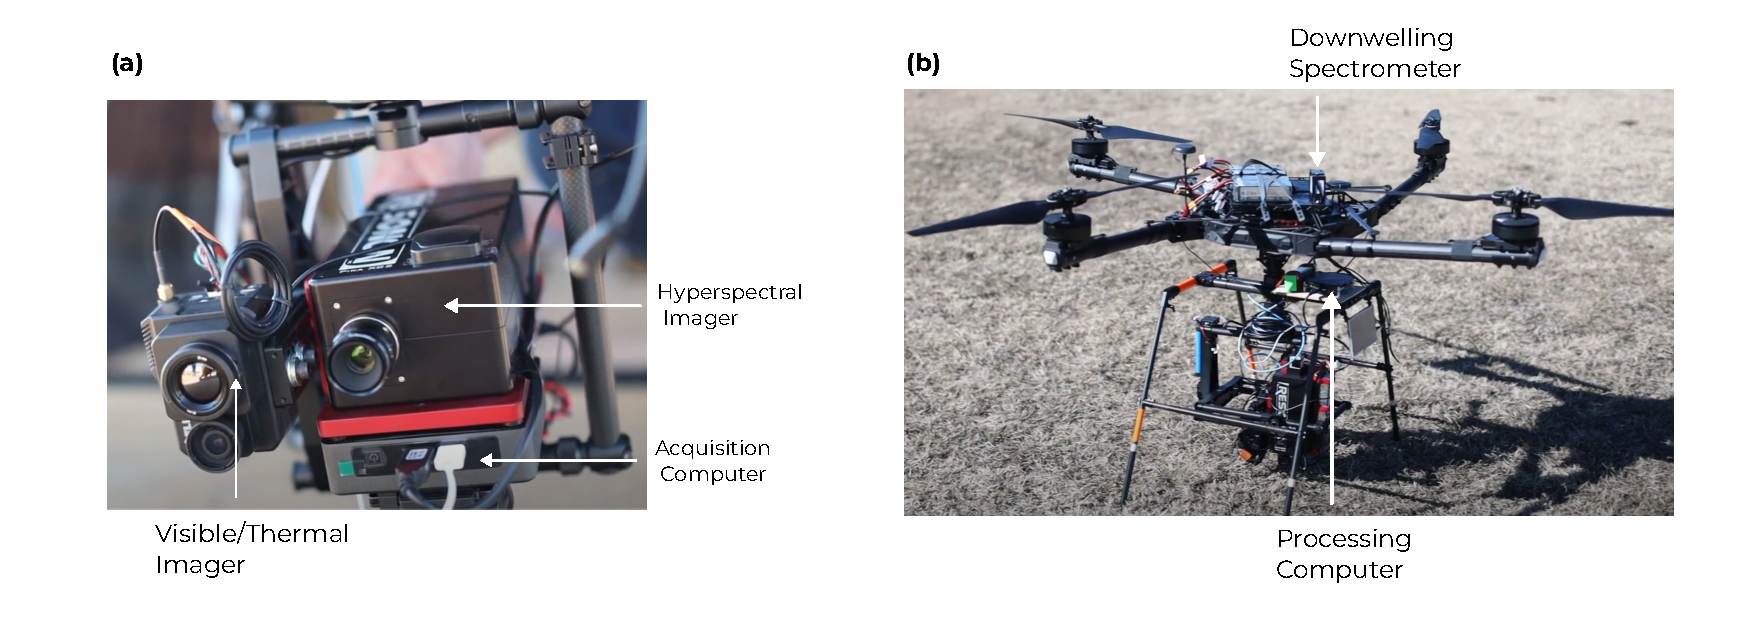
\includegraphics[width=\columnwidth]{paper/figures/materials-and-methods/annotated-drone.pdf}
\caption{Configuration of the UAV: (\textbf{a}) the hyperspectral imager and acquisition computer. (\textbf{b}) the assembled UAV with secondary processing computer and (upward facing) downwelling irradiance spectrometer. \label{fig:drone-components}}
\end{figure} 

To effectively utilize the spectra collected by our UAV, we must account for the variability of the incident light illuminating the water and transform the raw hyperspectral data cubes from their native \textit{imaging reference frame} to a chosen coordinate system compatible with the data collected by the USV. This procedure is illustrated in Figure~\ref{fig:hsi-pipeline}.

\begin{figure}[H]
\begin{adjustwidth}{-\extralength}{0cm}
\centering
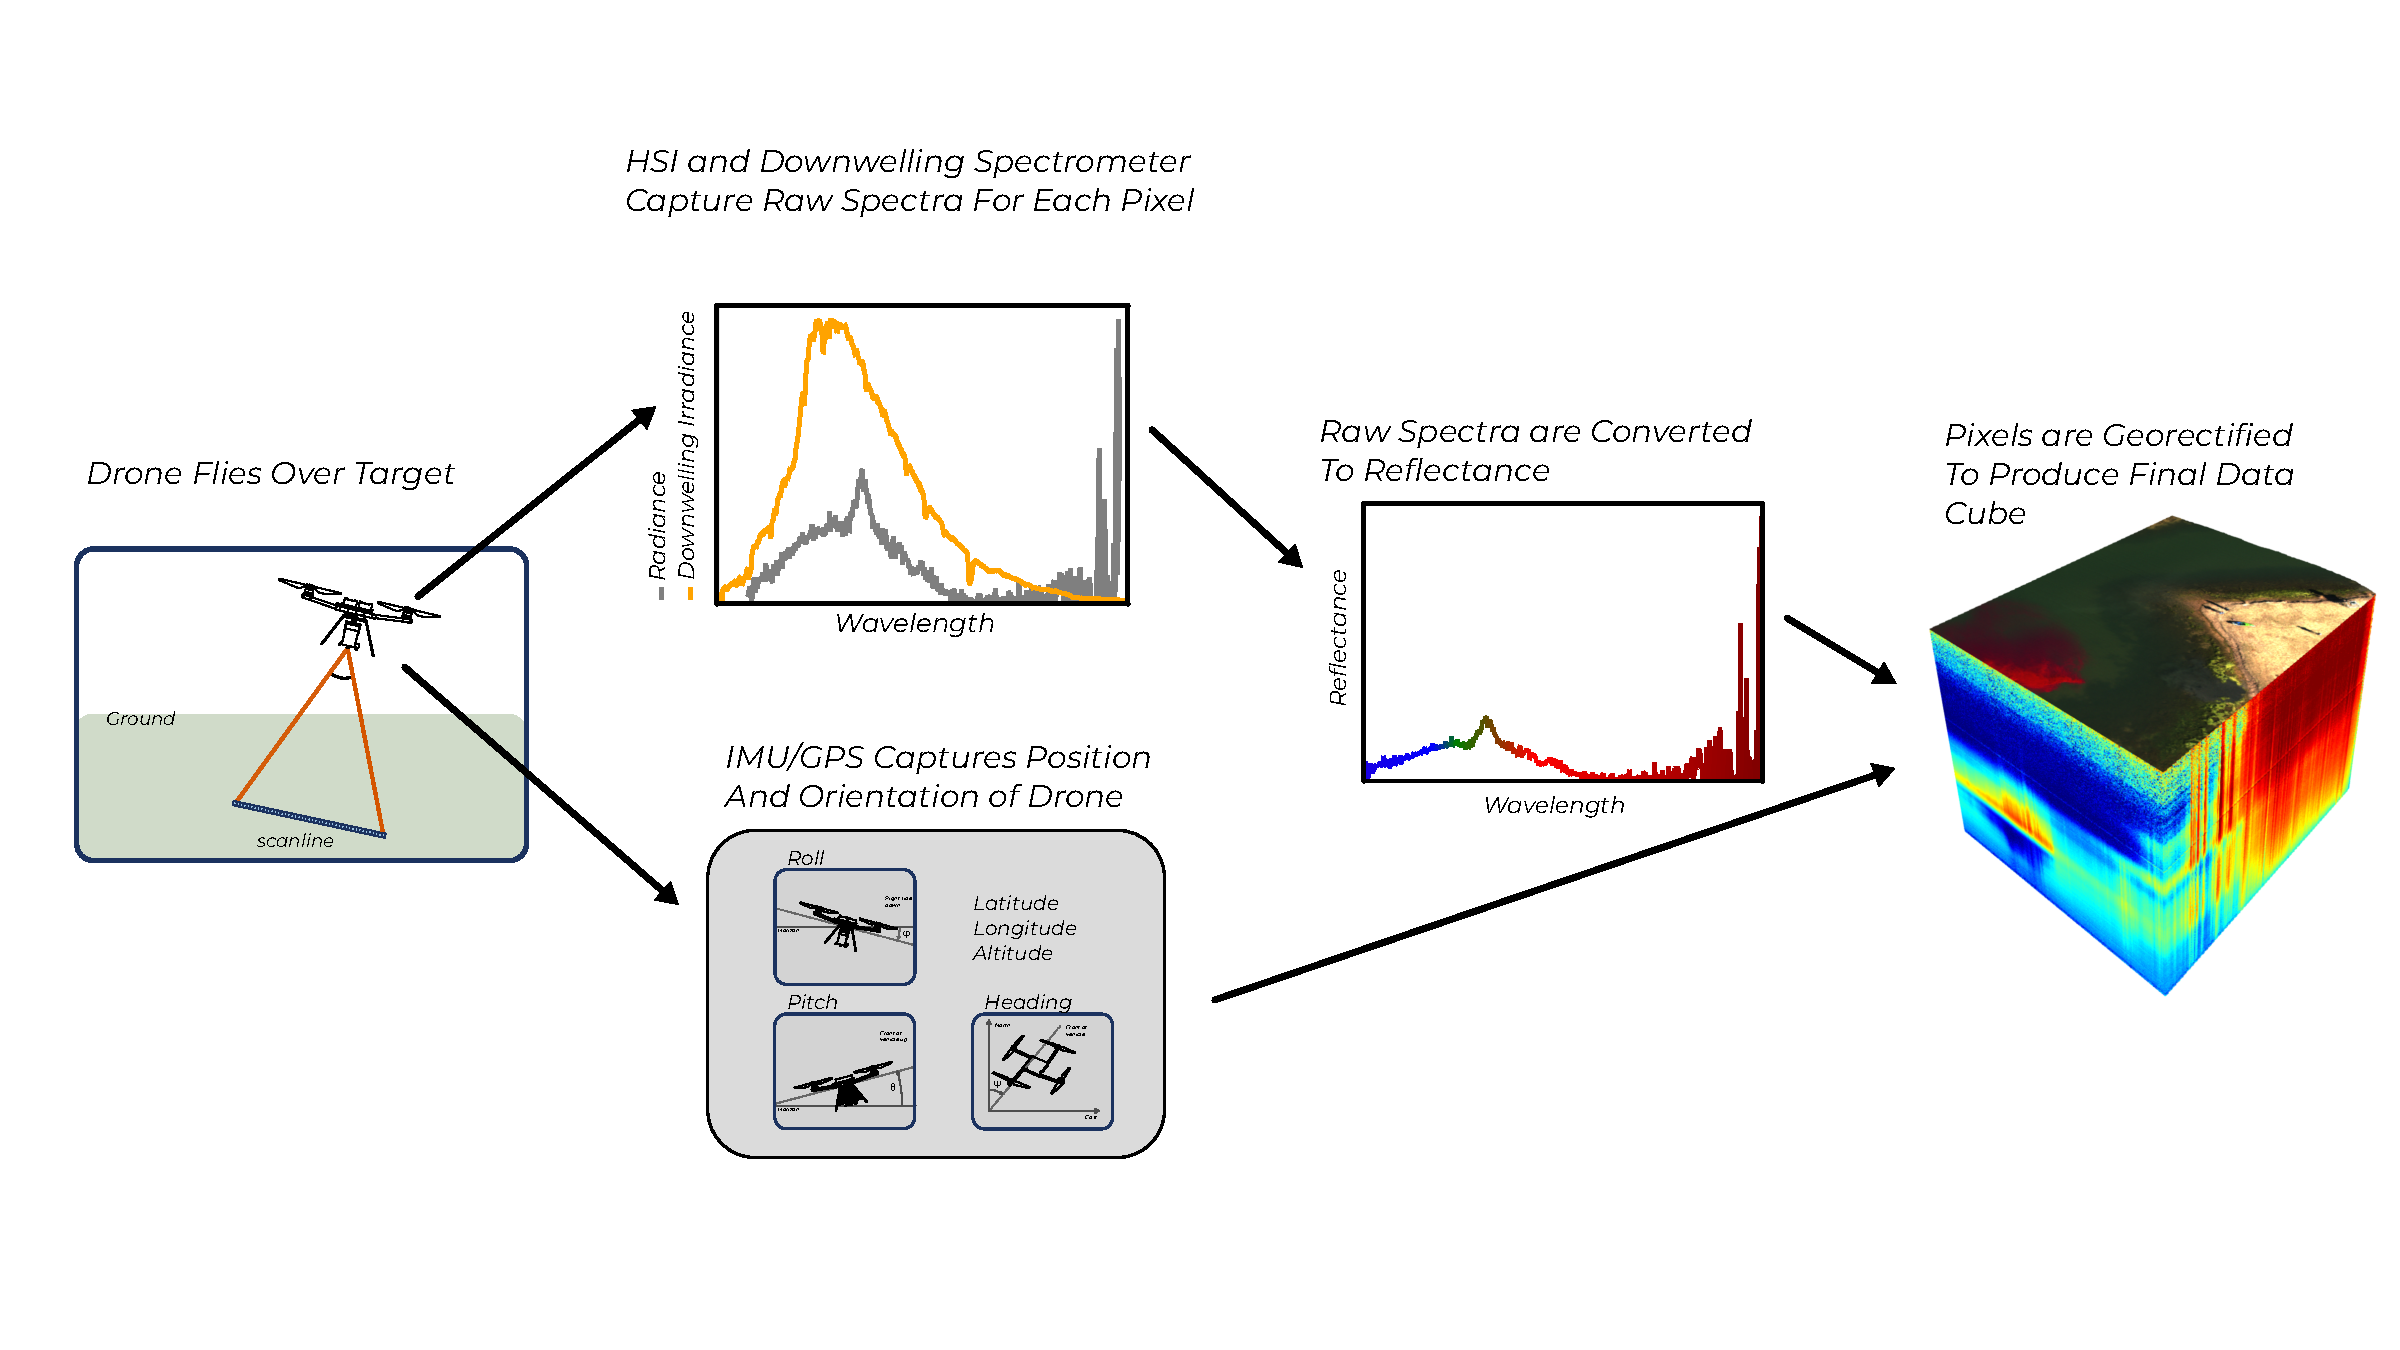
\includegraphics[width=16cm]{paper/figures/materials-and-methods/pipeline-figure-2.pdf}
\end{adjustwidth}
\caption{Hyperspectral Image Processing: Hyperspectral datacubes are collected one scan-line at a time (left). By utilizing downwelling irradiance spectra we convert each pixel from spectral radiance to reflectance. By using orientation and position data from the on-board GPS and INS, we georeference each pixel to assign it a latitude and longitude on the ground. The final data product is a georectified hyperspectral reflectance data cube visualized at the right. \label{fig:hsi-pipeline}}
\end{figure}  

The hyperspectral imager utilized in our robot team is in a so-called \textit{pushbroom} configuration, that is, each image captured by the drone is formed one scan-line at a time as the UAV flies. Each scan-line consists of 1600 pixels for which incoming light is diffracted into 462 wavelength bins. In the collection software, a regular cutoff of 1000 lines is chosen so that each resulting \textit{image} forms a array of size 462$\times$1600$\times$1000 called a \textit{hyperspectral data cube}. Initially, the sampled spectra are in units of spectral radiance (measured in microflicks) however this does not account for the variability of incident light illuminating the water. To this end, we convert the hyperspectral data cubes into units of reflectance by utilizing the skyward-facing downwelling irradiance spectrometer (see Figure~\ref{fig:drone-components}). When our camera is normal to this surface, then the reflectance is given by
\begin{equation}
    R(\lambda) = \pi L(\lambda)/E_d(\lambda)
\end{equation}
where $L$ is the spectral radiance, $E_d$ is the downwelling irradiance, and a factor of $\pi$ steradians results from assuming the water surface is Lambertian (diffuse) \cite{reflectance-conversion}. We will address the impact of this assumption in Section~\ref{sec:discussion}.

Having converted the hyperspectral data cube to units of reflectance, we must also georeference each pixel into a geographic coordinate system so that each image pixel can be assigned a latitude and longitude corresponding to the location on the ground from which it was sampled. During our three surveys, the UAV was flown at an altitude of ~50 m above the water. At this scale, the surface is essentially flat so that the hyperspectral data cube can be reliably georectified without the need for an on-board digital elevation map (DEM). We adopt the approach outlined in \cite{GeorectificationMuller, GeorectificationBaumker, GeorectificationMostafa} whereby each scan-line is georeferenced using the known field of view (30.8 $\deg$) together with the position and orientation of the UAV as provided by the on-board GPS/INS. After a sequence of coordinate transformations, pixel coordinates are obtained in the relevant UTM zone (in meters). The resulting image is then re-sampled to a final output resolution. For these collections a resolution of 10 cm was utilized, however this can be increased to reduce the processing time for real-time applications. Finally, the UTM coordinates are transformed to latitude and longitude for easy comparison with in-situ data collected by the USV. The final result is a georectified hyperspectral reflectance data cube. In Figure~\ref{fig:hsi-infographic} we visualize one such data cube, highlighting a selection of exemplar pixel spectra from the scene as well as the incident downwelling irradiance spectrum. A pseudo-color image is generated (plotted on the top of the data cube) to illustrate the scene.

\begin{figure}[H]
\begin{adjustwidth}{-\extralength}{0cm}
\centering
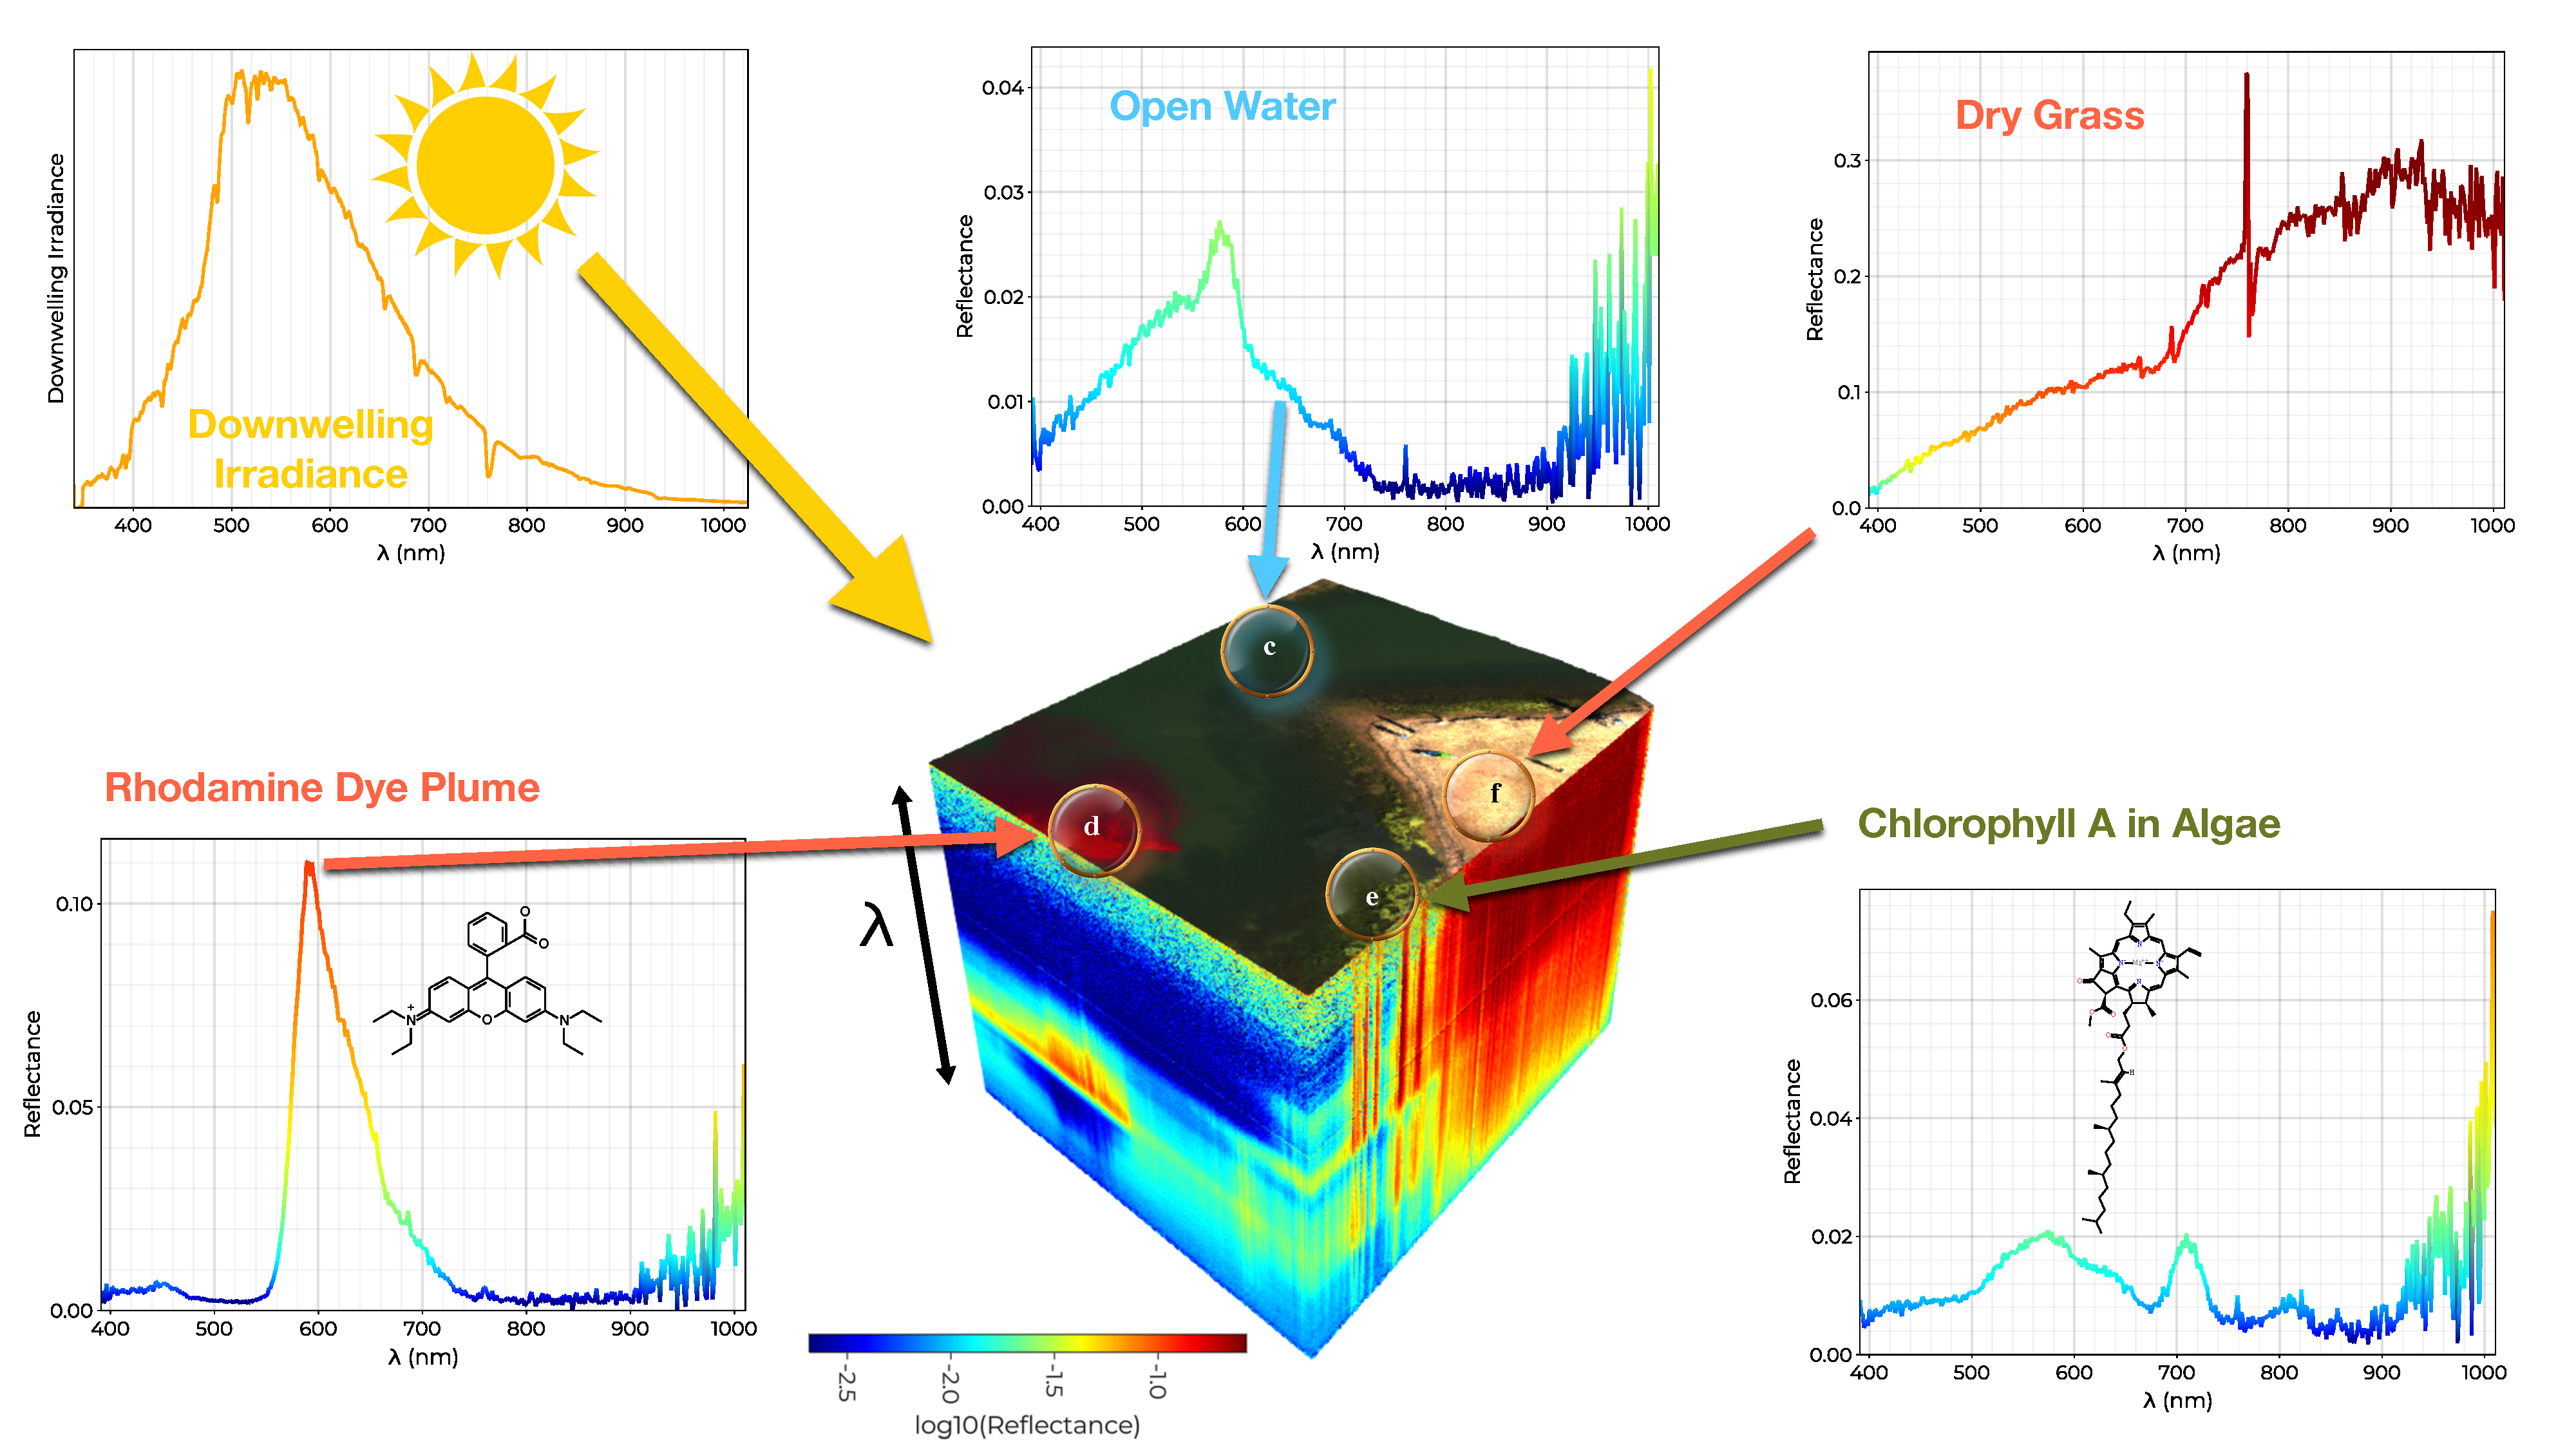
\includegraphics[width=15.5cm]{paper/figures/materials-and-methods/HyperSpectralInfoGraphic.pdf}
\end{adjustwidth}
\caption{A georectified reflectance data cube is visualized (center) with the $\log10$-reflectance along the z axis and a pseudo-color image on the top. In the top left we visualize the downwelling irradiance spectrum (the incident light). The surrounding plots showcase exemplar pixel reflectance spectra for open water, dry grass, algae, and a rhodamine dye plume used to test the system.\label{fig:hsi-infographic}}
\end{figure}  

The above processing pipeline was implemented using the Julia programming language, a just-in-time compiled language with native multi-theading support \cite{julia-1}. By running this pipeline on the on-board processing computer, we are able to process the collected hyperspectral data cubes in near real time. This feature is critical for time-sensitive applications where we need to quickly asses if an area is safe and can not afford to wait to download and post-process collected imagery \textit{after} a flight.

\subsection{Data Collection and Training Set Curation}

Data were collected using the robot team at a site in north Texas across three observation periods in the fall of 2020. For each collection period, the UAV first completed two wide surveys of the lake capturing multiple hyperspectral data cubes. Subsequently, the the USV sampled across the lake, collecting in-situ reference measurements. Each of these reference measurements was then collocated with individual pixel spectra where the USV track overlapped with UAV pixels. To account for any time-delays in the values measured by the in-situ instruments and to account for the fact the the USV is larger than the final resolution of our resampled HSI, each in-siture measurent is associated with a 3$\times$3 grid of HSI pixels, that is, a 30 cm $\times$ 30 cm square. These combined data form a tabular data set on which we seek use to train regression models; pixel spectra form input features and each separate USV sensor forms a distinct target variable. Together, this combined data set contains over 130,000 records.

Each collection was performed near solar noon to maximize the amount of incident sunlight illuminating the water, however, to account for any potential variation in lighting conditions between data cubes, we augment the training set with additional features including the drone viewing geometry (roll, pitch, heading) and solar illumination geometry (solar azimuth, solar elevation, solar zenith) as well as the total at-pixel intensity (before refelctance conversion), the total downwelling intensity, and the drone altitude. Feature engineering is performed to add a additional spectral indices utilizing combinations of specific wavelength bands like the normalized difference vegetation index (NDVI), normalized difference water index (NDWI), simple ratio (SR), photochemical reflectance index (PRI), and more as described in \cite{envi_vegetation_indices, thenkabail2018hyperspectral,kaufman1992atmospherically, SpectralIndexWheat}. A comprehensive list of these added features is provided in supplementary table S1.

\subsection{Machine Learning Methods}

For each of the 17 target variables listed in Table~\ref{tab:sensors}, data were randomly partitioned into a 90:10 training/testing split resulting 120,350 training points and 13,372 holdout testing points. Using the MLJ machine learning framework, a variety of machine learning models compatible with the regression task were identified \cite{MLJ1}. This selection of models included linear regression (and it's variations), Gaussian Process Regression, shallow Neural Networks, and decision tree based models. Out of this set, Random Forest Regression from \cite{decision-trees} and a native Julia implementation of gradient boosted tree regression from the EvoTrees package were selected for their quick training and inference times. Both random forests and gradient boosted trees are ensembling techniques based on individual decision tree regressors \cite{decision-trees, random-forest, gradient-boosting}. These tree-based methods also enable an impurity based ranking of the relative \textit{importance} of each feature to the target predictions as described in \cite{rfr-orig,rfr-importance-ranking}. We use these feature rankings to identify the most impactful features and perform feature selection and reduction. 

The training procedure for each model is as follow: First, the model is trained using 6-fold cross validation on the training set with default hyperparameters. Feature importances for the trained model are then computed and the top 25 features are identified. A second, reduced-feature model is then trained using the same 6-fold cross validation technique to ensure an improvement in model performance. Next, each model is hyperparameter optimized using a random parameter search. Model performance is evaluated by computing out-of-fold values for the $R^2$ (coefficient of determination), as well as
\begin{align}
    \text{RMSE} &= \sqrt{\frac{\sum\limits_{i=1}^N (\hat{y}_i-y_i)^2}{N}}, \\
    \text{MAE} &= \frac{\sum\limits_{i=1}^N \lvert \hat{y}_i - y_i \vert}{N},
\end{align}
where RMSE is the root-mean-square error, and MAE is the mean absolute error between true values $y_i$ and predictions $\hat{y}_i$.

Having identified the model with the best out-of-fold performance, we proceed to train the final hyperparameter optimized model on the full training set. To assess the uncertainty of the final model's predictions, we employ Inductive Conformal Prediction as described in \cite{conformal-prediction-1, conformal-prediction-2, conformal-prediction-3, conformal-prediction-4}. To do this, the training set is further partitioned so that we obtain an additional validation hold out set with the split chosen to achieve a 80:10:10 training, validation, and testing ratio. This resulting validation set contains >10,000 records which \cite{conformal-prediction-2} suggests to be more than sufficient for most cases. 

The hyperparameter optimized model is trained on the full training set. We then compute a set of nonconformity scores on the validation set using an uncertainty heuristic, in this case, the absolute error
\begin{equation}
    s_i = s(X_i, y_i) = \lvert f(X_i) - y_i \rvert = \lvert \hat{y}_i - y_i \rvert
\end{equation}
where $f(X_i)=\hat{y}_i$ denotes the trained ML model applied to the $i^{th}$ calibration record. These n-many scores are sorted, and the interval half width $d$ is computed as the $\frac{\lceil(\alpha)(n+1) \rceil}{n}$ quantile of this set in order to achieve a coverage of $\alpha$ on the calibration set. Predictions intervals for new data are then formed as $f(X)\pm d$. For this study, we have chosen a coverage of $\alpha=0.9$ corresponding to a 90\% confidence interval. Finally, each of these resulting hyperparameter optimized models is evaluated on the previously untouched testing set.


%%%%%%%%%%%%%%%%%%%%%%%%%%%%%%%%%%%%%%%%%%
\section{Results}

The results of fitting our hyperparameter optimized models are listed in Table~\ref{tab:fit-results}. For each model, the $R^2$, RMSE, and MAE were evaluated using 6-fold cross validation. We observe considerable 

\begin{table}[H]
  \caption{Summary of fitting statistics for each target measurement. Models were evaluated using 6-fold cross validation on the training set. The estimated uncertainty is evaluated using conformal prediction so that a prediction $\hat{y}\pm \Delta y$ achieves 90\% coverage on the calibration holdout set. The empirical coverage is the percentage of predictions in the testing set that fall within the confidence interval determined by conformal prediction. The final column shows the best performing model. \label{tab:fit-results}}
  \begin{adjustwidth}{-\extralength}{0cm}
  \newcolumntype{C}{>{\centering\arraybackslash}X}
  \begin{tabularx}{\fulllength}{CCCCCCC}
    \toprule
    \textbf{Target (units)} & \textbf{$\text{R}^2$} & \textbf{RMSE} & \textbf{MAE} & \textbf{Estimated Uncertainty} & \textbf{Empirical Coverage (\%)} & \textbf{Model*}\\
    \midrule
    Temperature (°C) & 1.0 ± 1.98e-5 & 0.0398 ± 0.00096 & 0.0267 ± 0.00055 &  ± 0.061 & 89.8 &\\
    Conductivity ($\mu$S/cm) & 0.999 ± 2.17e-5 & 0.853 ± 0.0114 & 0.55 ± 0.00564 &  ± 1.3 & 89.8\\
    $\mathrm{Ca}^{2+}$ (mg/l) & 0.999 ± 3.53e-5 & 0.423 ± 0.0101 & 0.243 ± 0.00552 &  ± 0.59 & 89.7\\
    Dissolved Oxygen (mg/l) & 0.999 ± 3.17e-5 & 0.0705 ± 0.000984 & 0.0467 ± 0.000418 &  ± 0.11 & 89.8\\
    Salinity (PSU) & 0.998 ± 0.000129 & 0.000759 ± 1.8e-5 & 0.000265 ± 6.1e-6 &  ± 0.00051 & 89.6\\
    $\mathrm{Cl^-}$ (mg/l) & 0.994 ± 0.000441 & 1.15 ± 0.0418 & 0.578 ± 0.00534 &  ± 1.4 & 90.3\\
    $\mathrm{Na^+} (mg/l)$ & 0.992 ± 0.000309 & 6.17 ± 0.134 & 2.85 ± 0.0536 &  ± 7.2 & 89.9\\
    Tryptophan (ppb) & 0.991 ± 0.00038 & 0.188 ± 0.00404 & 0.112 ± 0.00149 &  ± 0.26 & 89.9\\
    pH & 0.991 ± 0.000327 & 0.0177 ± 0.000295 & 0.0109 ± 6.56e-5 &  ± 0.024 & 89.9\\
    Blue-Green Algae [Phycoerythrin] (ppb) & 0.981 ± 0.00186 & 1.72 ± 0.0947 & 0.608 ± 0.0218 &  ± 1.4 & 90.2\\
    $\mathrm{NO_3^-} (mg/l-N)$ & 0.968 ± 0.00203 & 0.0308 ± 0.00113 & 0.0146 ± 0.000256 &  ± 0.043 & 89.9\\
    CDOM (ppb) & 0.966 ± 0.00228 & 0.464 ± 0.0195 & 0.144 ± 0.00449 &  ± 0.22 & 89.3\\
    Chlorophyll A ($\mu$g/l) & 0.924 ± 0.00645 & 1.29 ± 0.0667 & 0.359 ± 0.0079 &  ± 0.73 & 90.2\\
    Optical Brighteners (ppb) & 0.915 ± 0.00406 & 0.118 ± 0.00169 & 0.0568 ± 0.000218 &  ± 0.1 & 89.8\\
    Chlorophyll A with Red Excitation ($\mu$g/l) & 0.909 ± 0.00794 & 77.6 ± 3.91 & 15.6 ± 0.418 &  ± 25.0 & 90.5\\
    Crude Oil (ppb) & 0.906 ± 0.00606 & 0.588 ± 0.019 & 0.162 ± 0.00234 &  ± 0.23 & 89.7\\
    Turbidity (FNU) & 0.812 ± 0.0158 & 60.2 ± 2.61 & 6.98 ± 0.431 &  ± 3.4 & 89.5\\
    \bottomrule
  \end{tabularx}
  \end{adjustwidth}
  \noindent{\footnotesize{* RFR = Random Forest Regressor, ETR = EvoTree Regressor}}
\end{table}



\subsection{Physical Parameters}

\begin{figure}[H]
\begin{adjustwidth}{-\extralength}{0cm}
\centering
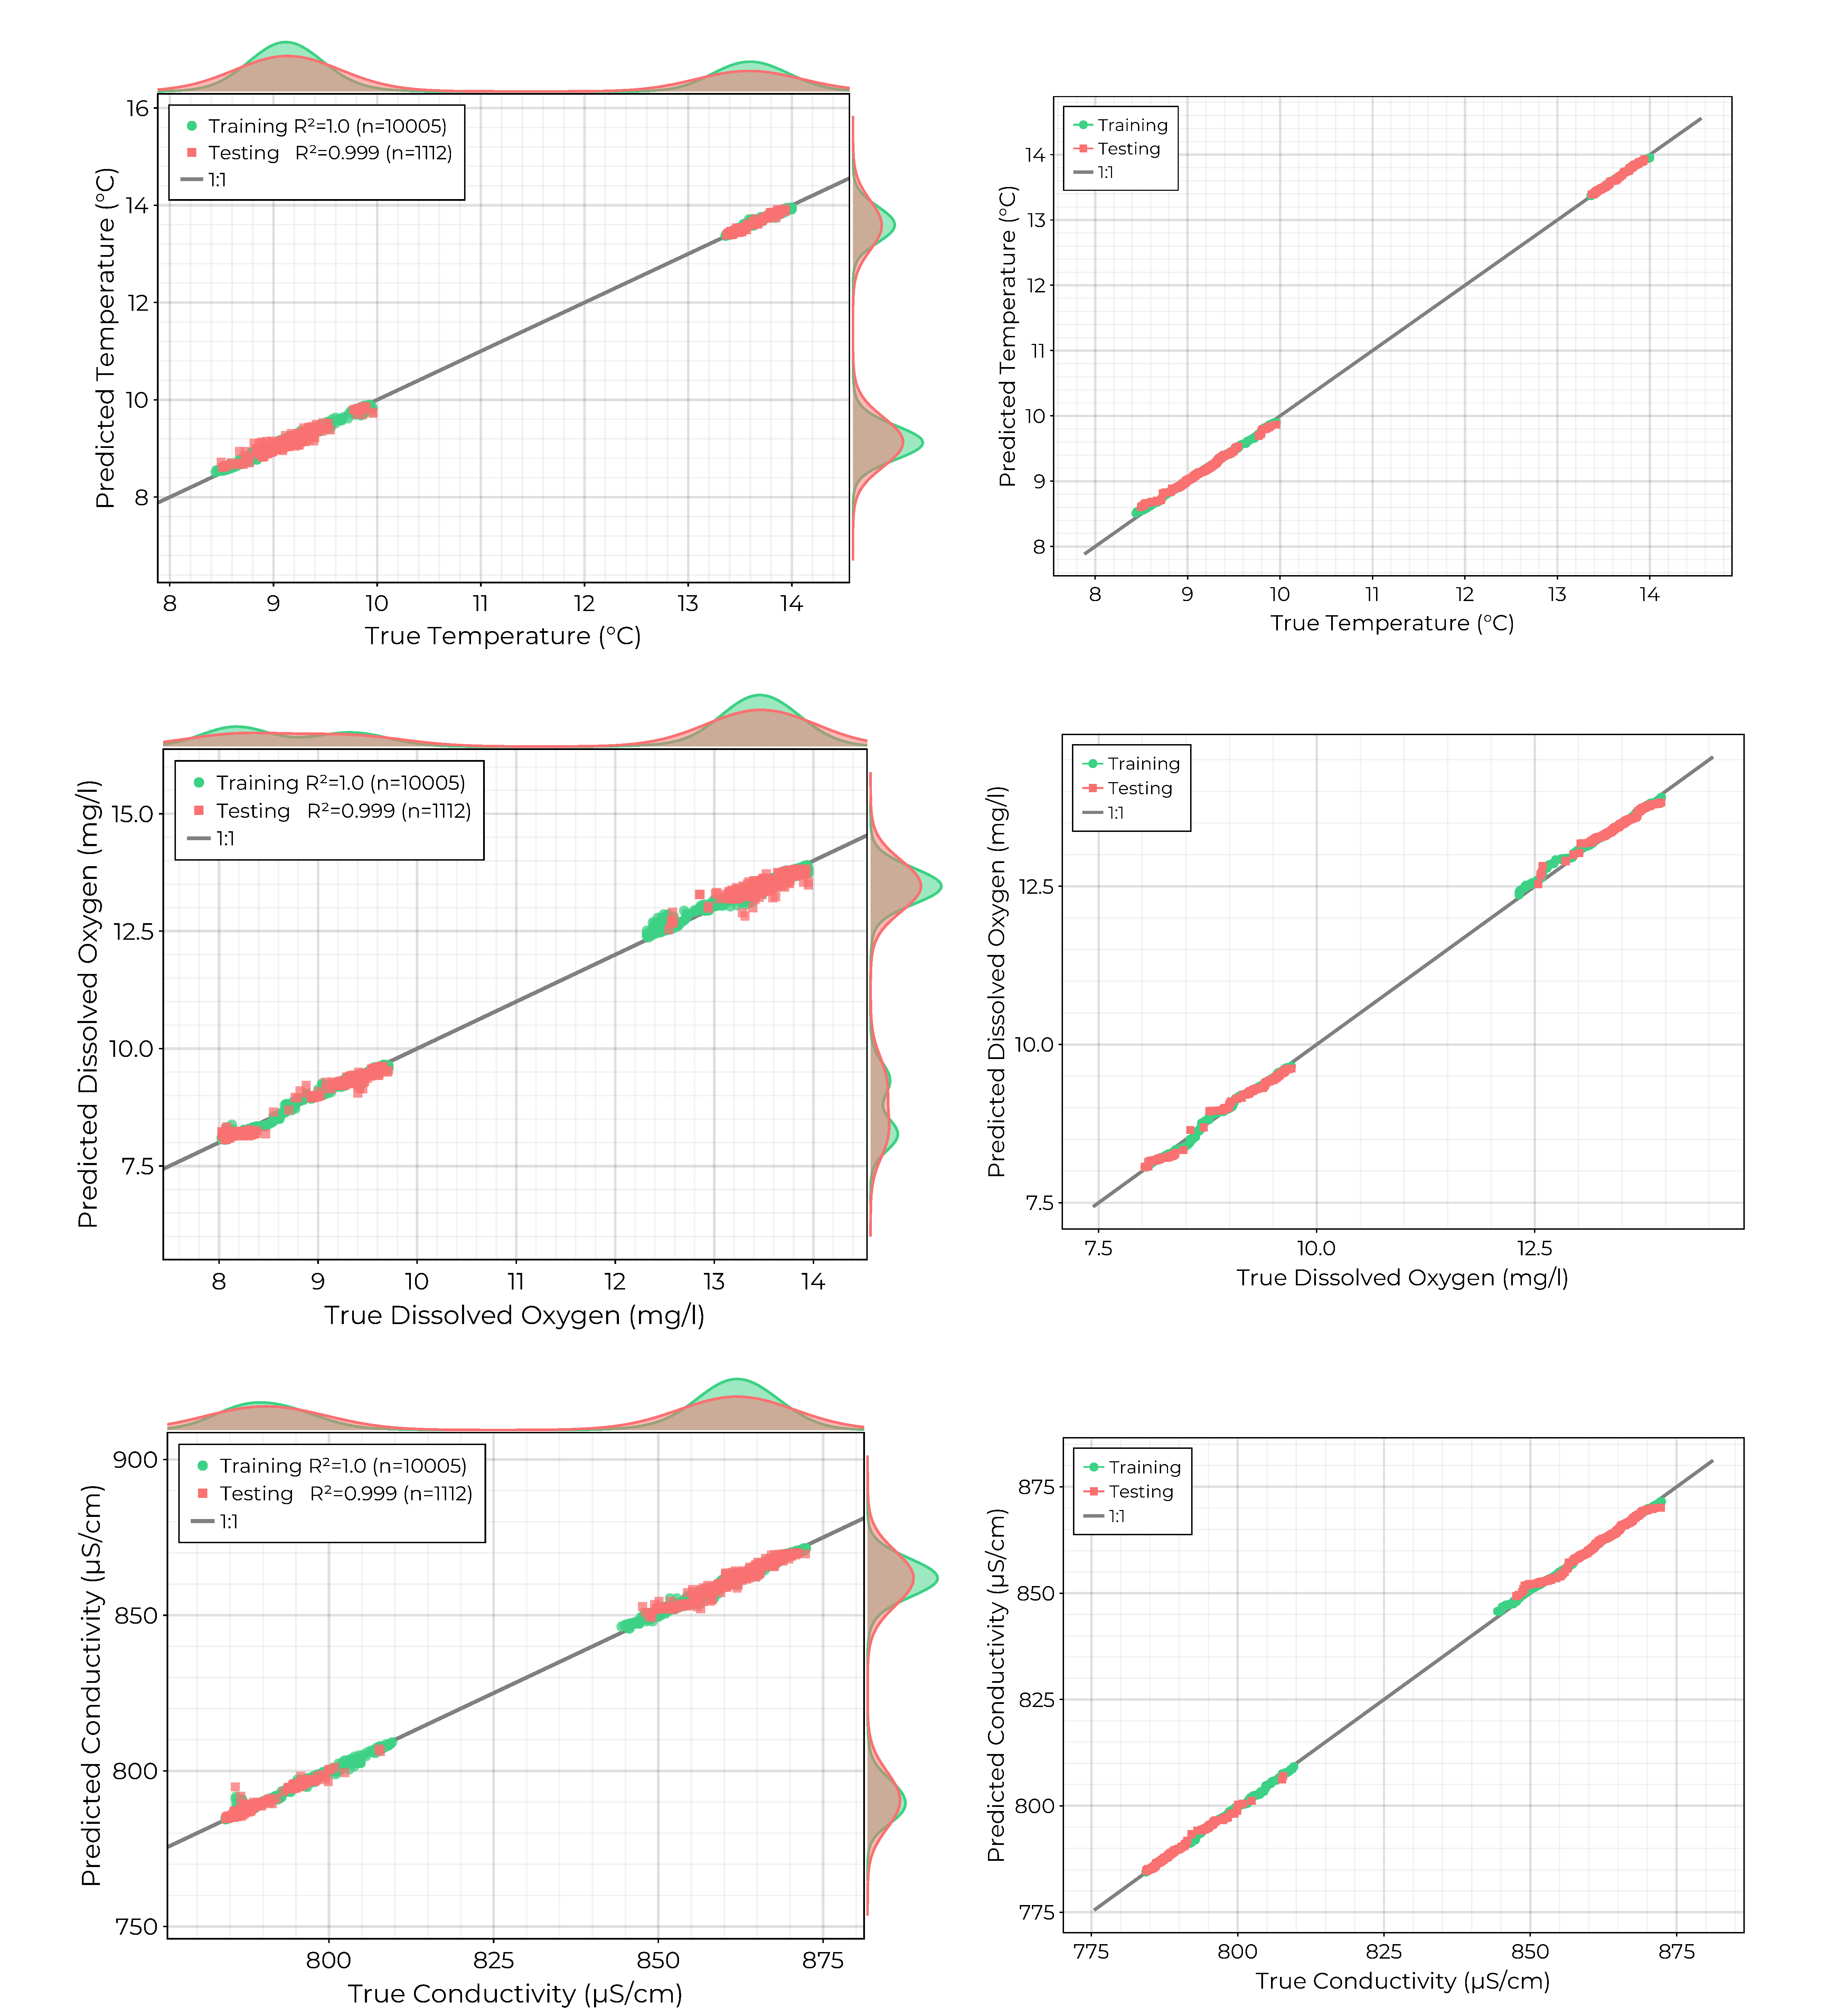
\includegraphics[width=16.0cm]{paper/figures/results/fits/physical-fitres.pdf}
\end{adjustwidth}
\caption{A visualization of the fitresults for three of the physical parameters we modeled. On the left is a scatterplot and on the right is plot of the associated quantiles.\label{fig:physical-fit}}
\end{figure}  

\begin{figure}[H]
\begin{adjustwidth}{-\extralength}{0cm}
\centering
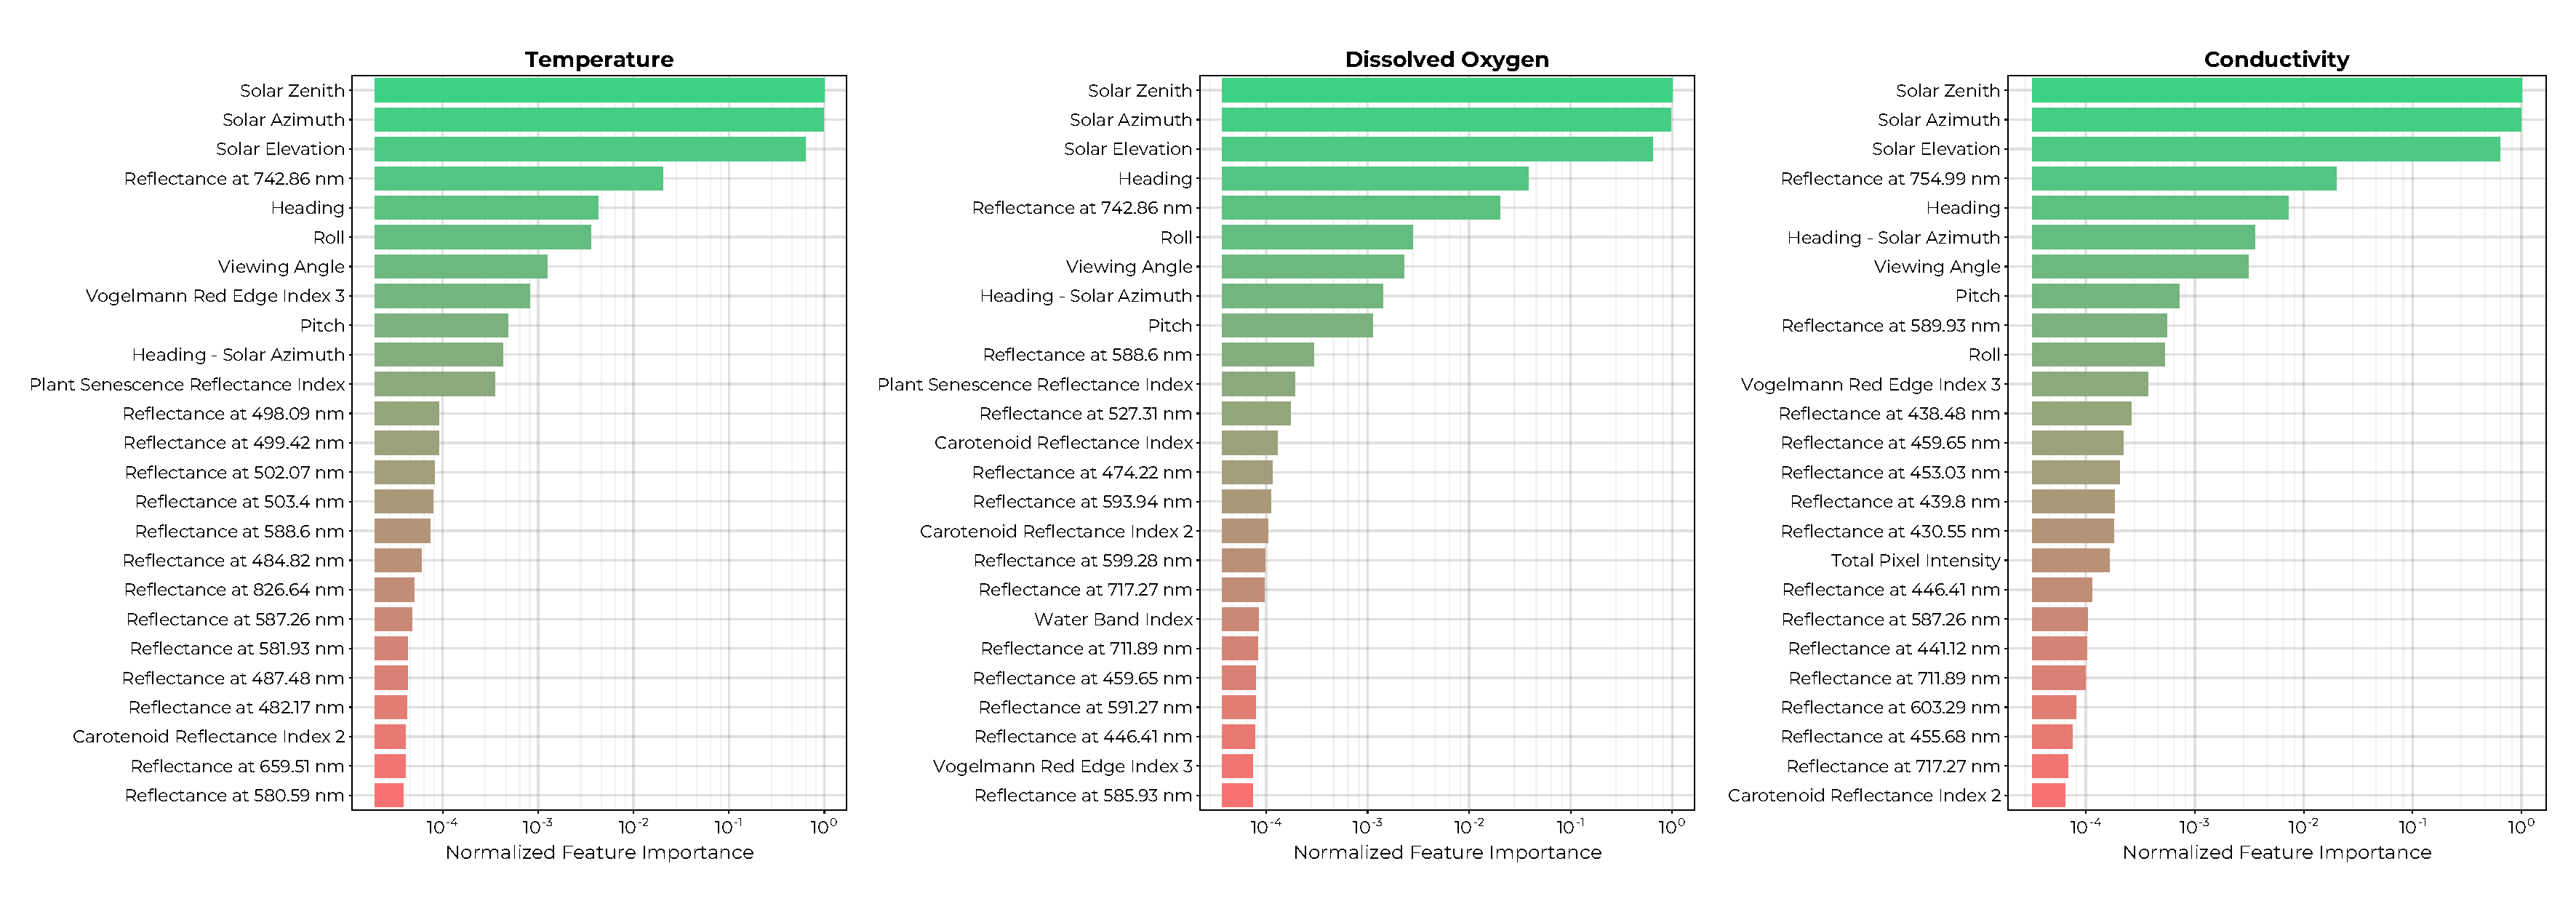
\includegraphics[width=18.0cm]{paper/figures/results/fits/physical-ranking.pdf}
\end{adjustwidth}
\caption{Ranked feature importances for the same three physical parameter models.\label{fig:physical-fit}}
\end{figure}  


\subsection{Ion Measurements}

\begin{figure}[H]
\begin{adjustwidth}{-\extralength}{0cm}
\centering
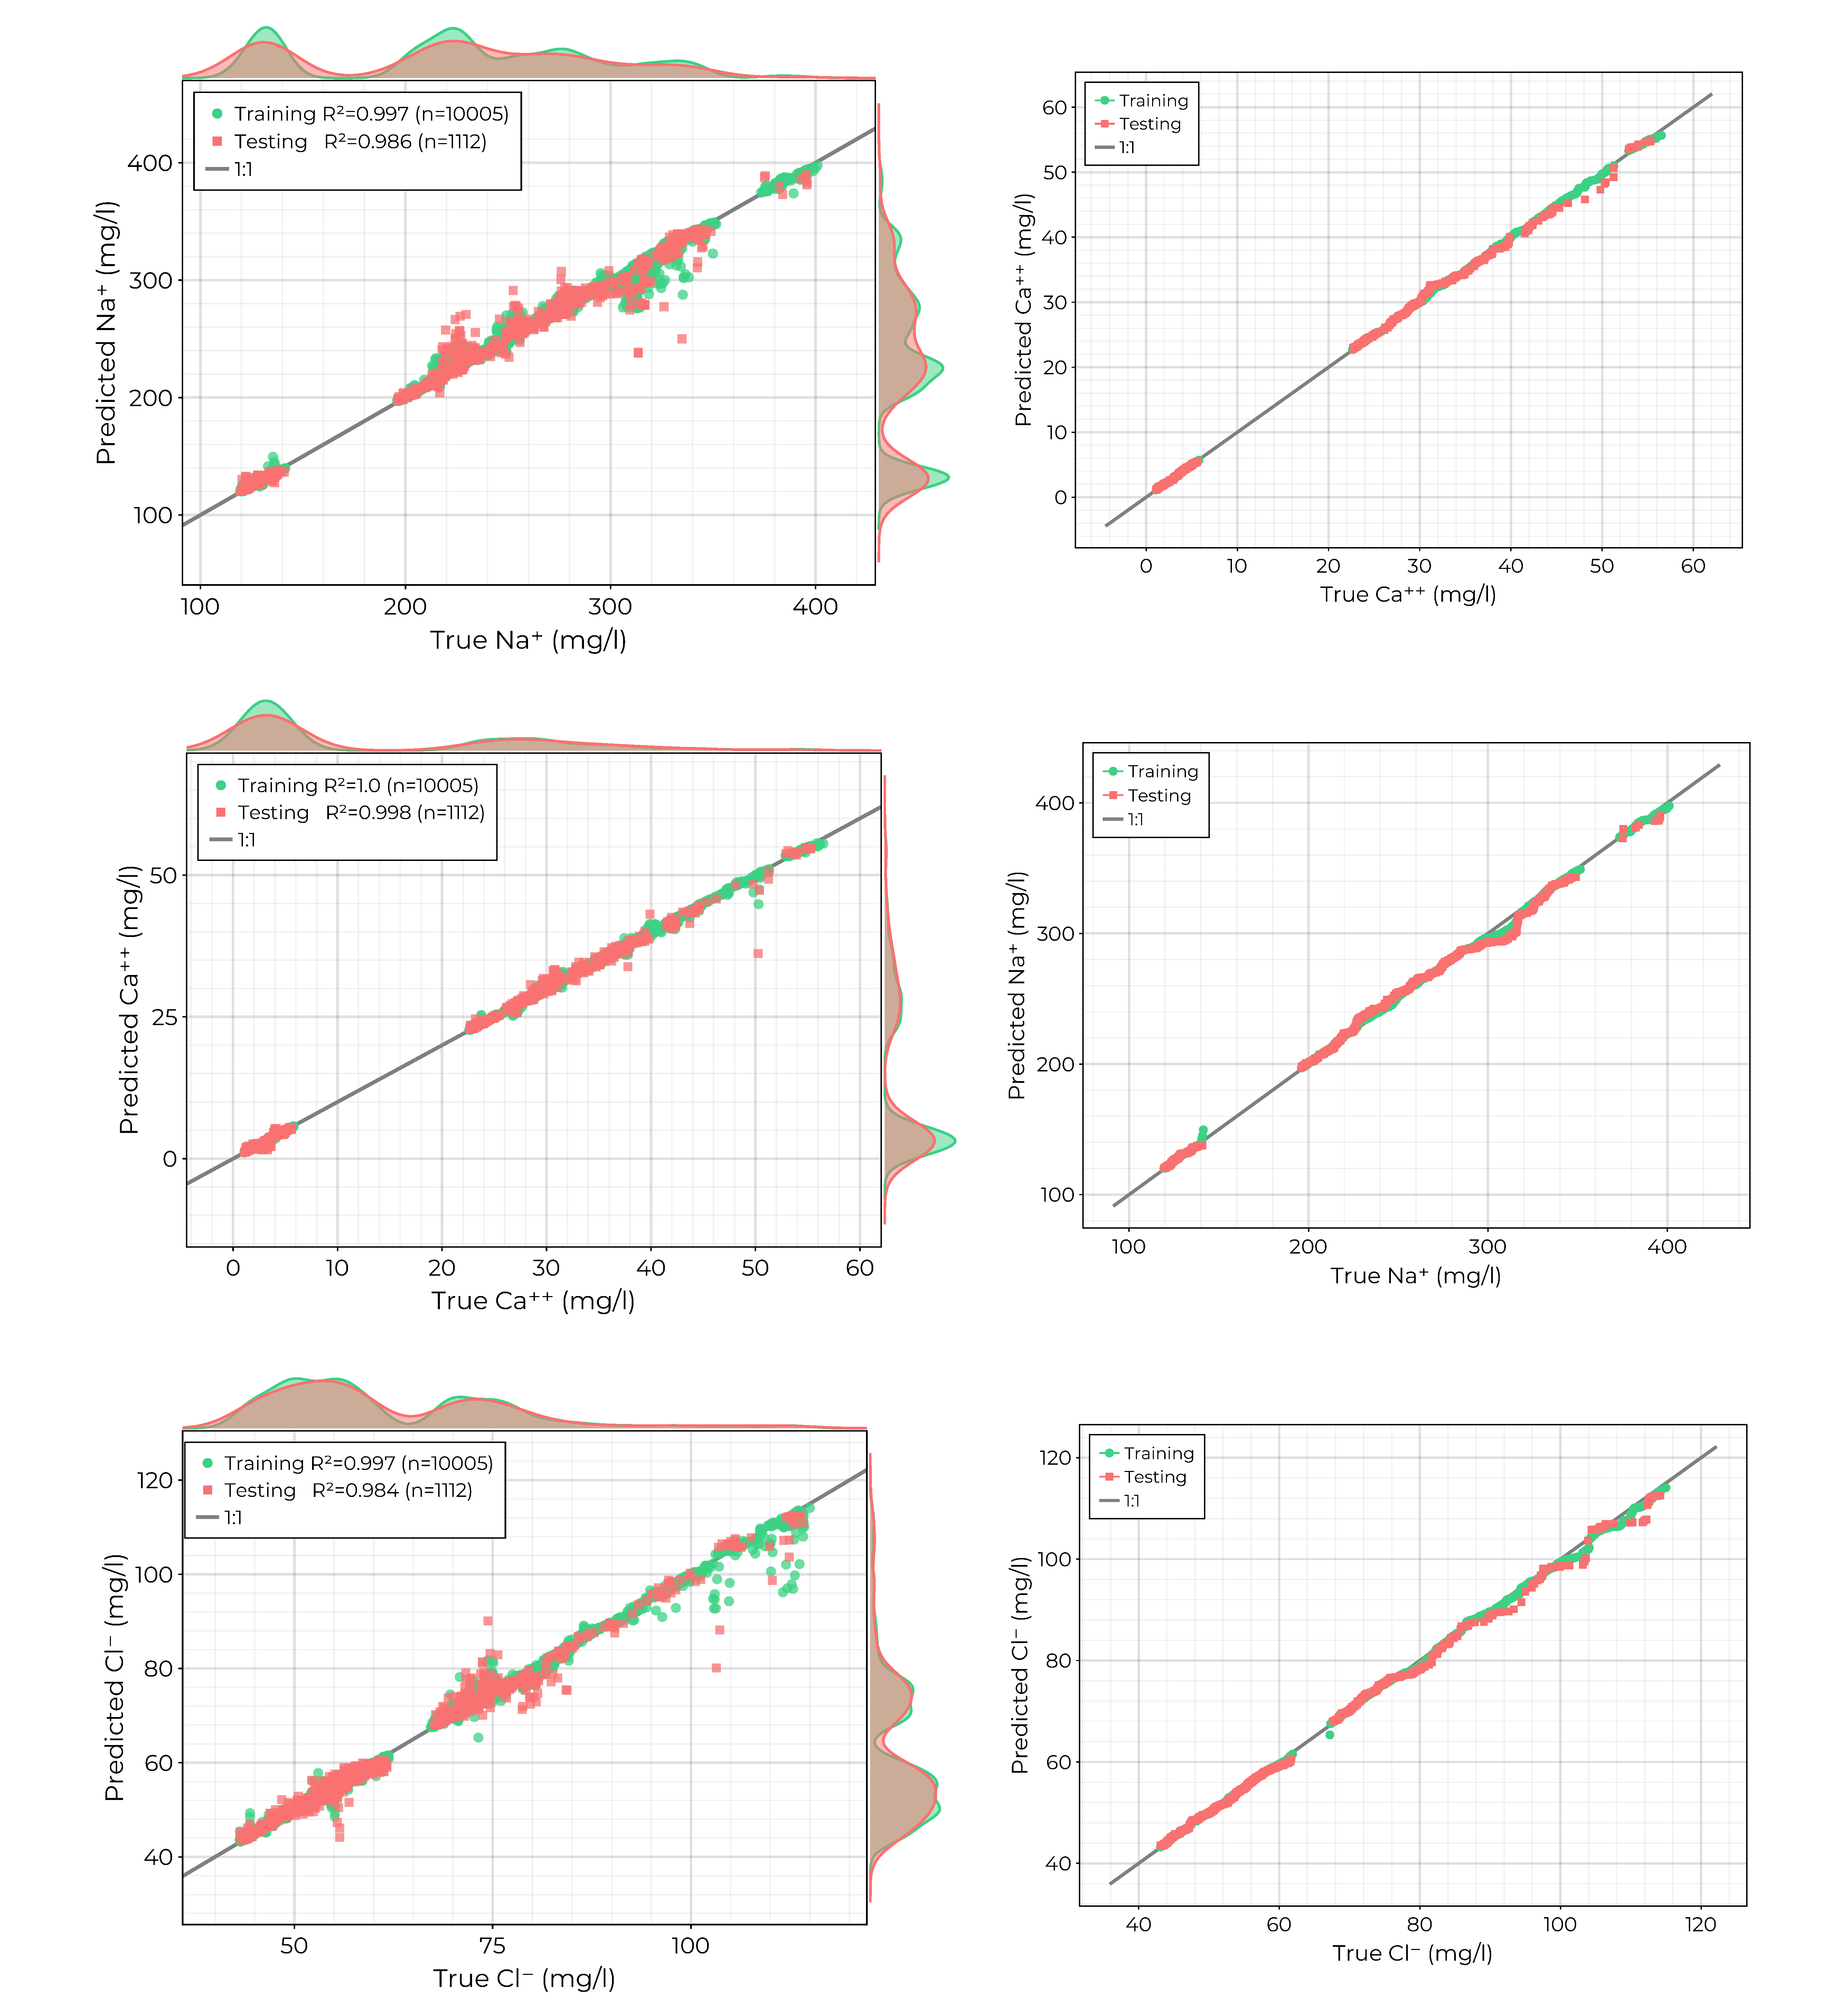
\includegraphics[width=16.0cm]{paper/figures/results/fits/ions-fitres.pdf}
\end{adjustwidth}
\caption{A visualization of the fitresults for three of the ion concentrations we modeled. On the left is a scatterplot and on the right is plot of the associated quantiles.\label{fig:ions-fit}}
\end{figure}  

\begin{figure}[H]
\begin{adjustwidth}{-\extralength}{0cm}
\centering
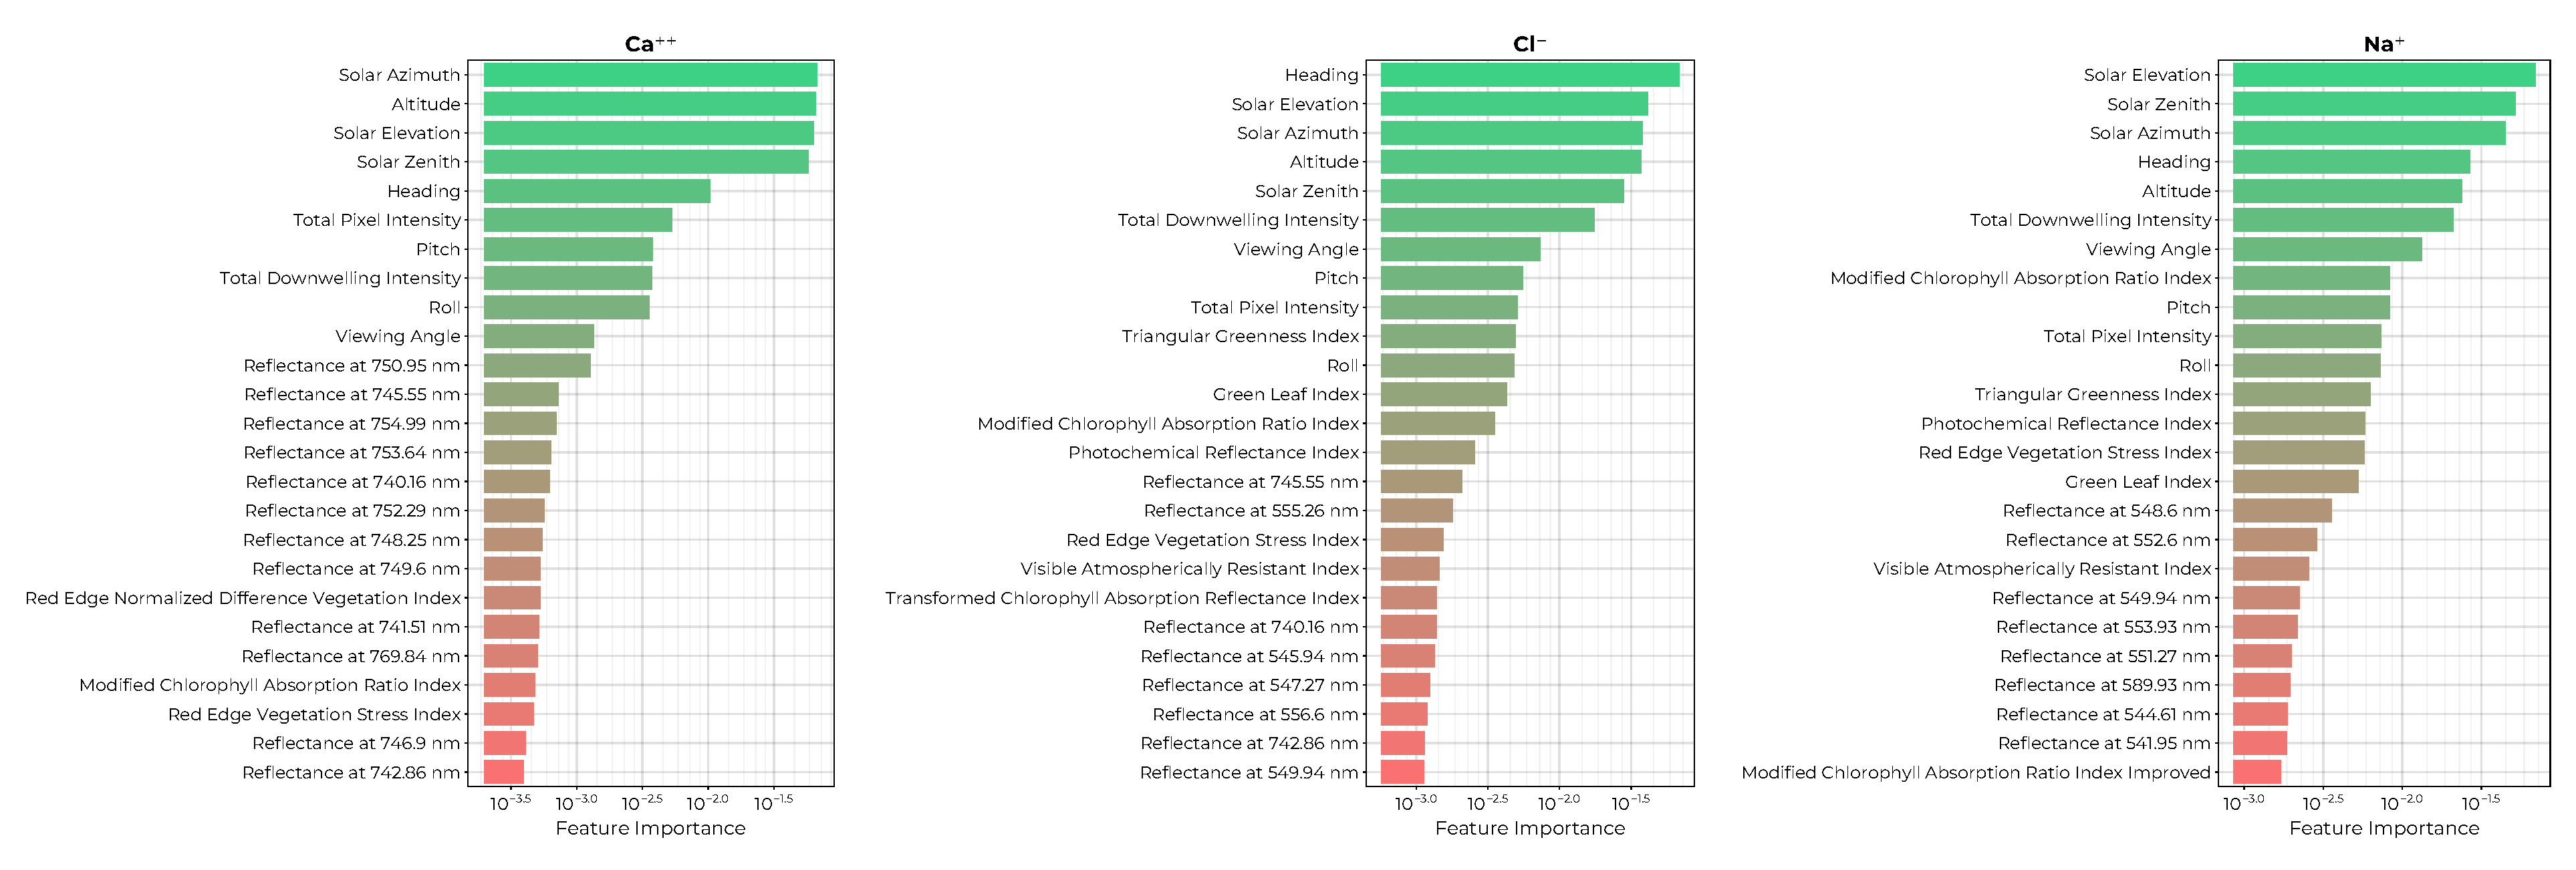
\includegraphics[width=18.0cm]{paper/figures/results/fits/ions-ranking.pdf}
\end{adjustwidth}
\caption{Ranked feature importances for the same three ion concentration models.\label{fig:ions-fit}}
\end{figure}  


\subsection{Biochemical Measurements}


\begin{figure}[H]
\begin{adjustwidth}{-\extralength}{0cm}
\centering
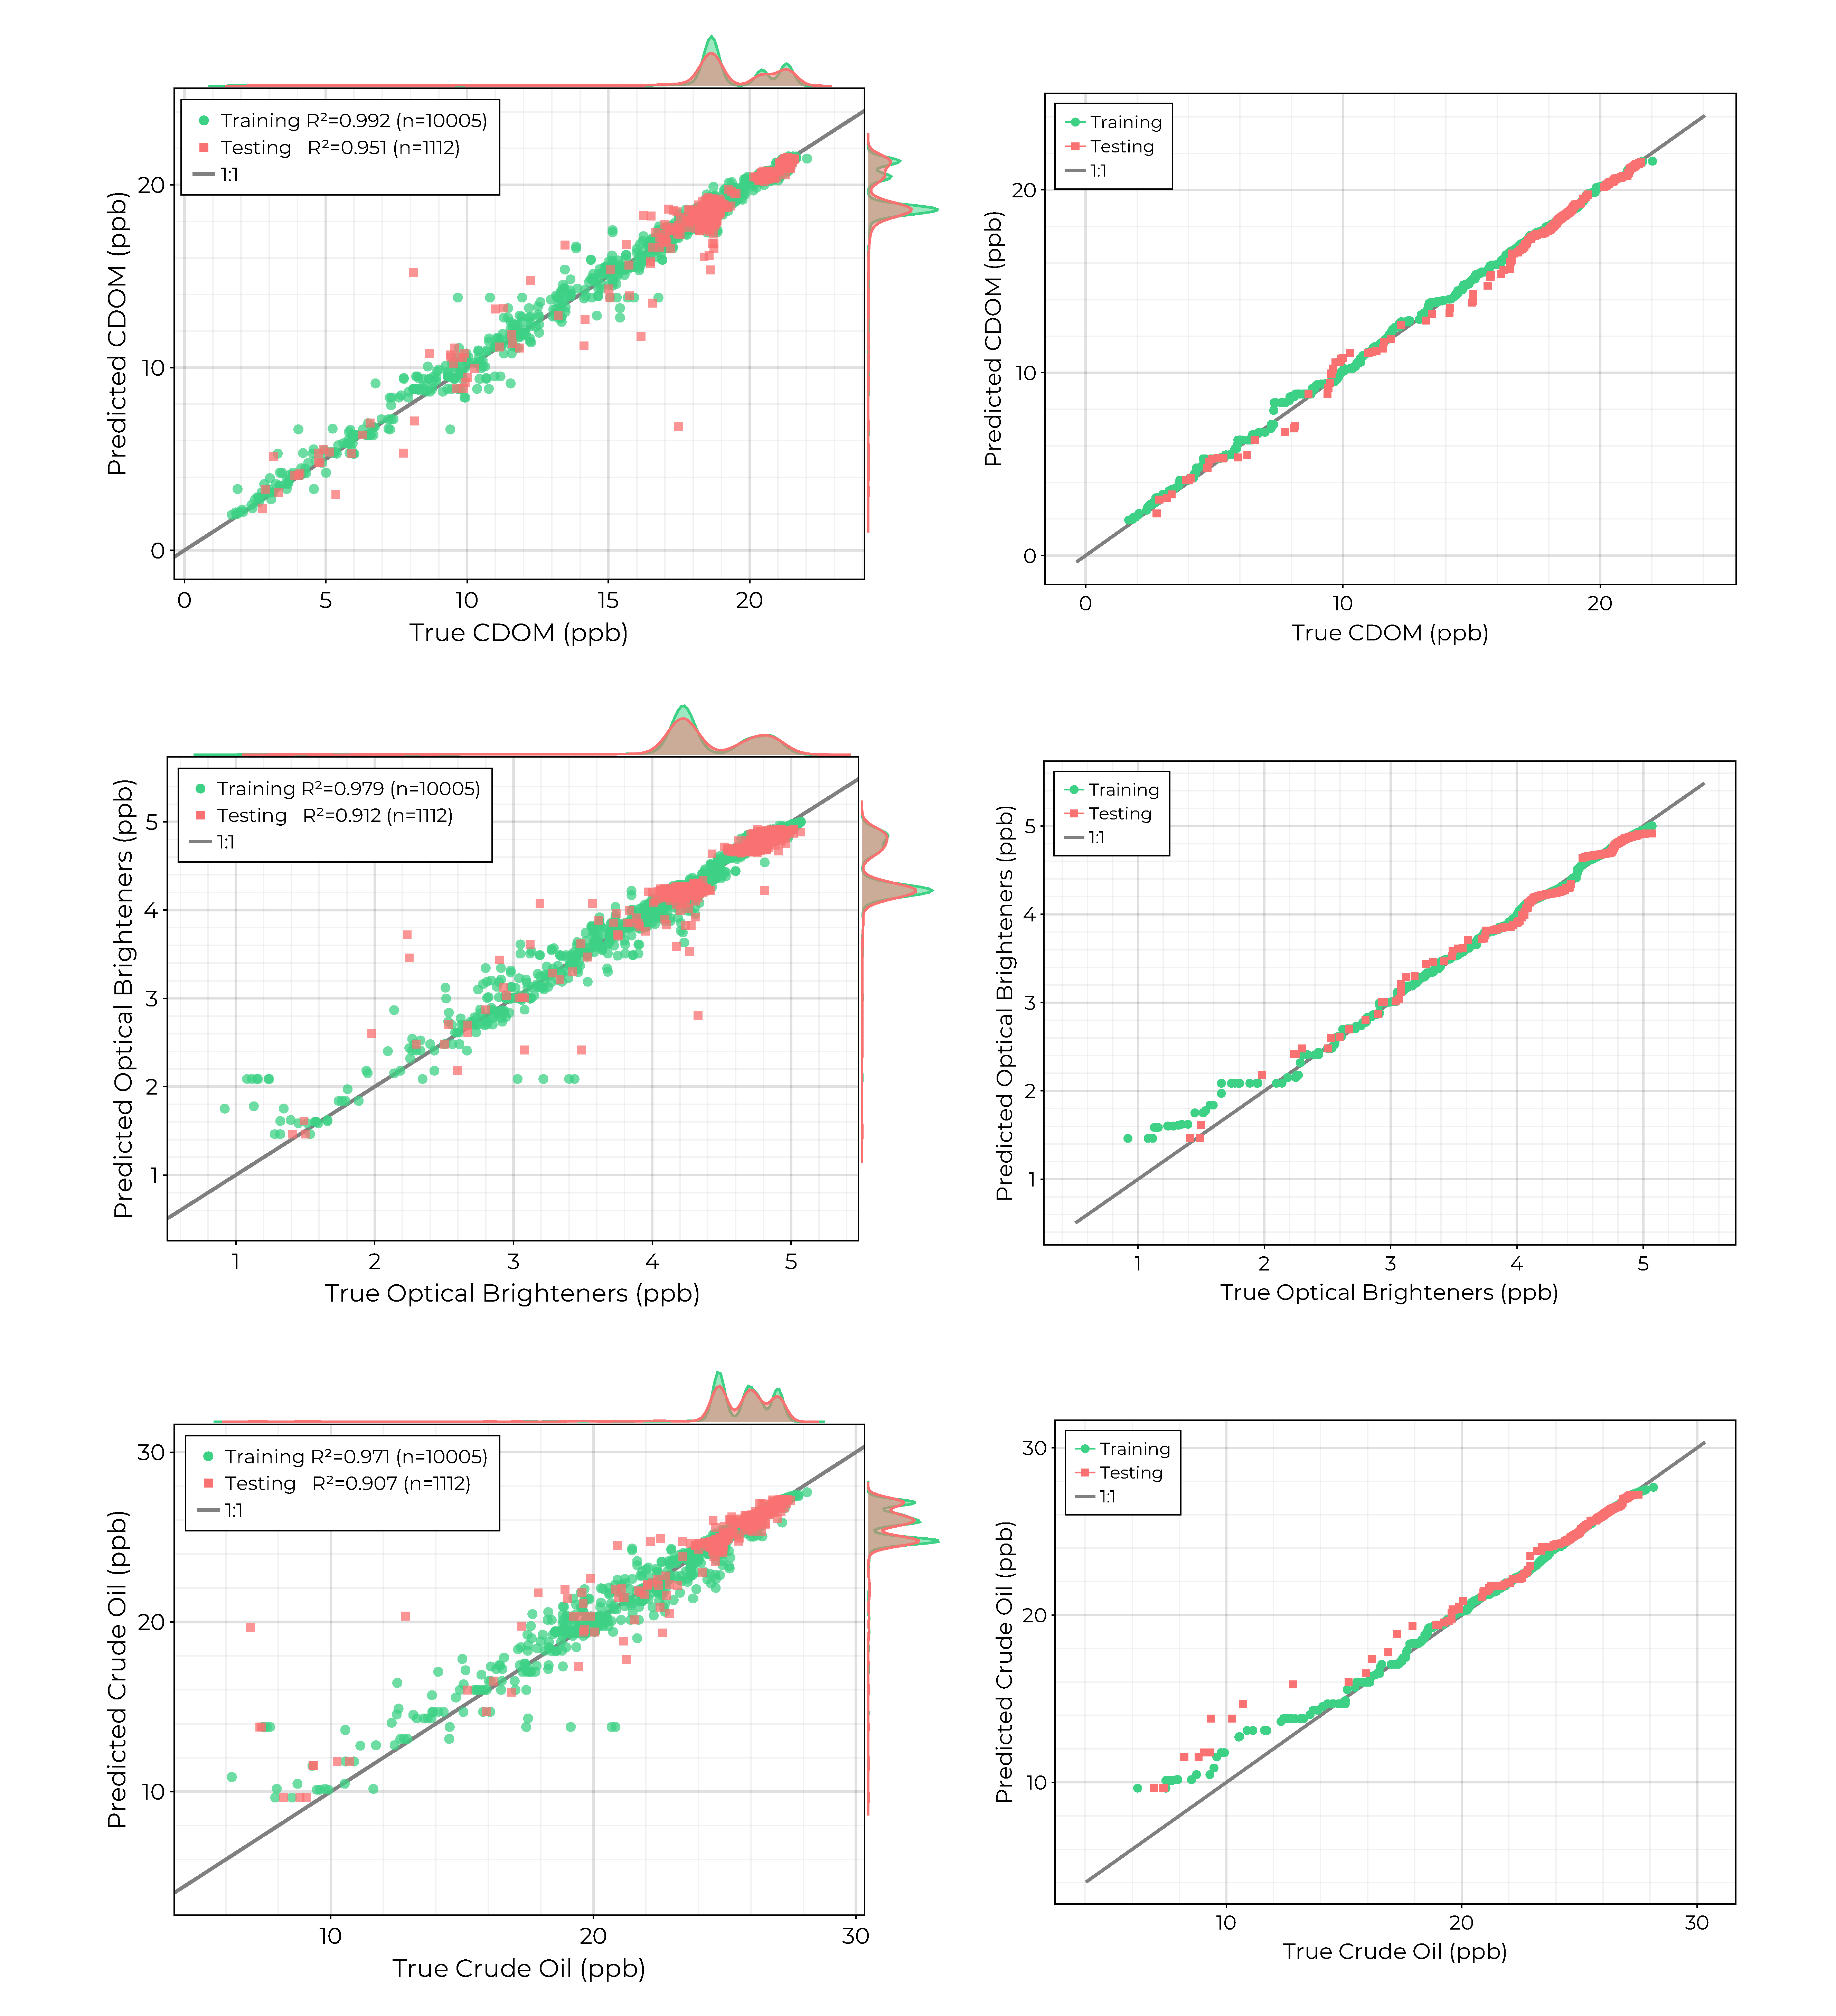
\includegraphics[width=16.0cm]{paper/figures/results/fits/chemical-fitres.pdf}
\end{adjustwidth}
\caption{A visualization of the fitresults for three of the chemical concentrations we modeled. On the left is a scatterplot and on the right is plot of the associated quantiles.\label{fig:chemicals-fit}}
\end{figure}  

\begin{figure}[H]
\begin{adjustwidth}{-\extralength}{0cm}
\centering
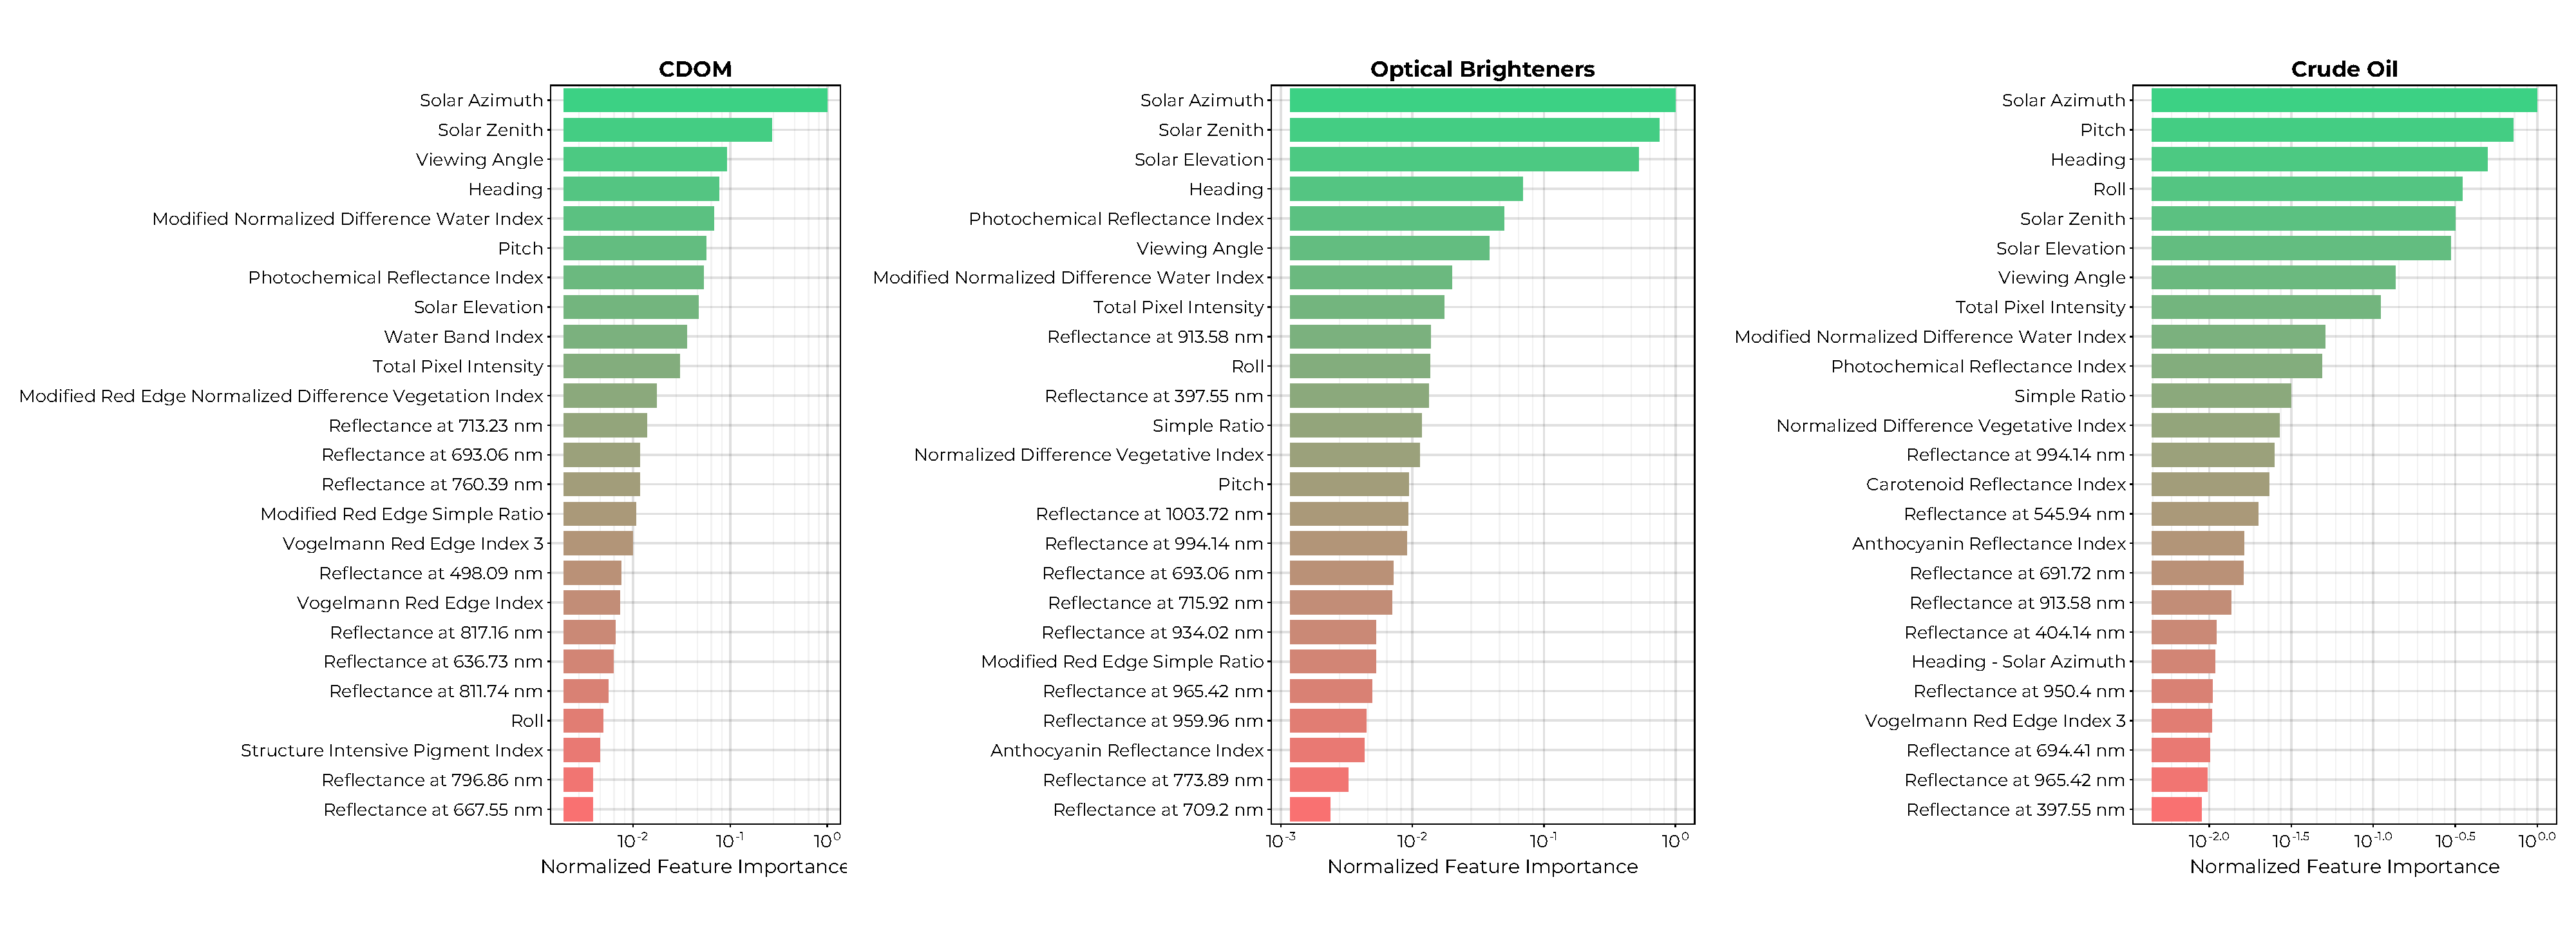
\includegraphics[width=18.0cm]{paper/figures/results/fits/chemical-ranking.pdf}
\end{adjustwidth}
\caption{Ranked feature importances for the same three chemical concentration models.\label{fig:chemicals-fit}}
\end{figure}  



\subsection{Mapping}

% Example of a figure that spans the whole page width. The same concept works for tables, too.
\begin{figure}[H]
\begin{adjustwidth}{-\extralength}{0cm}
\centering
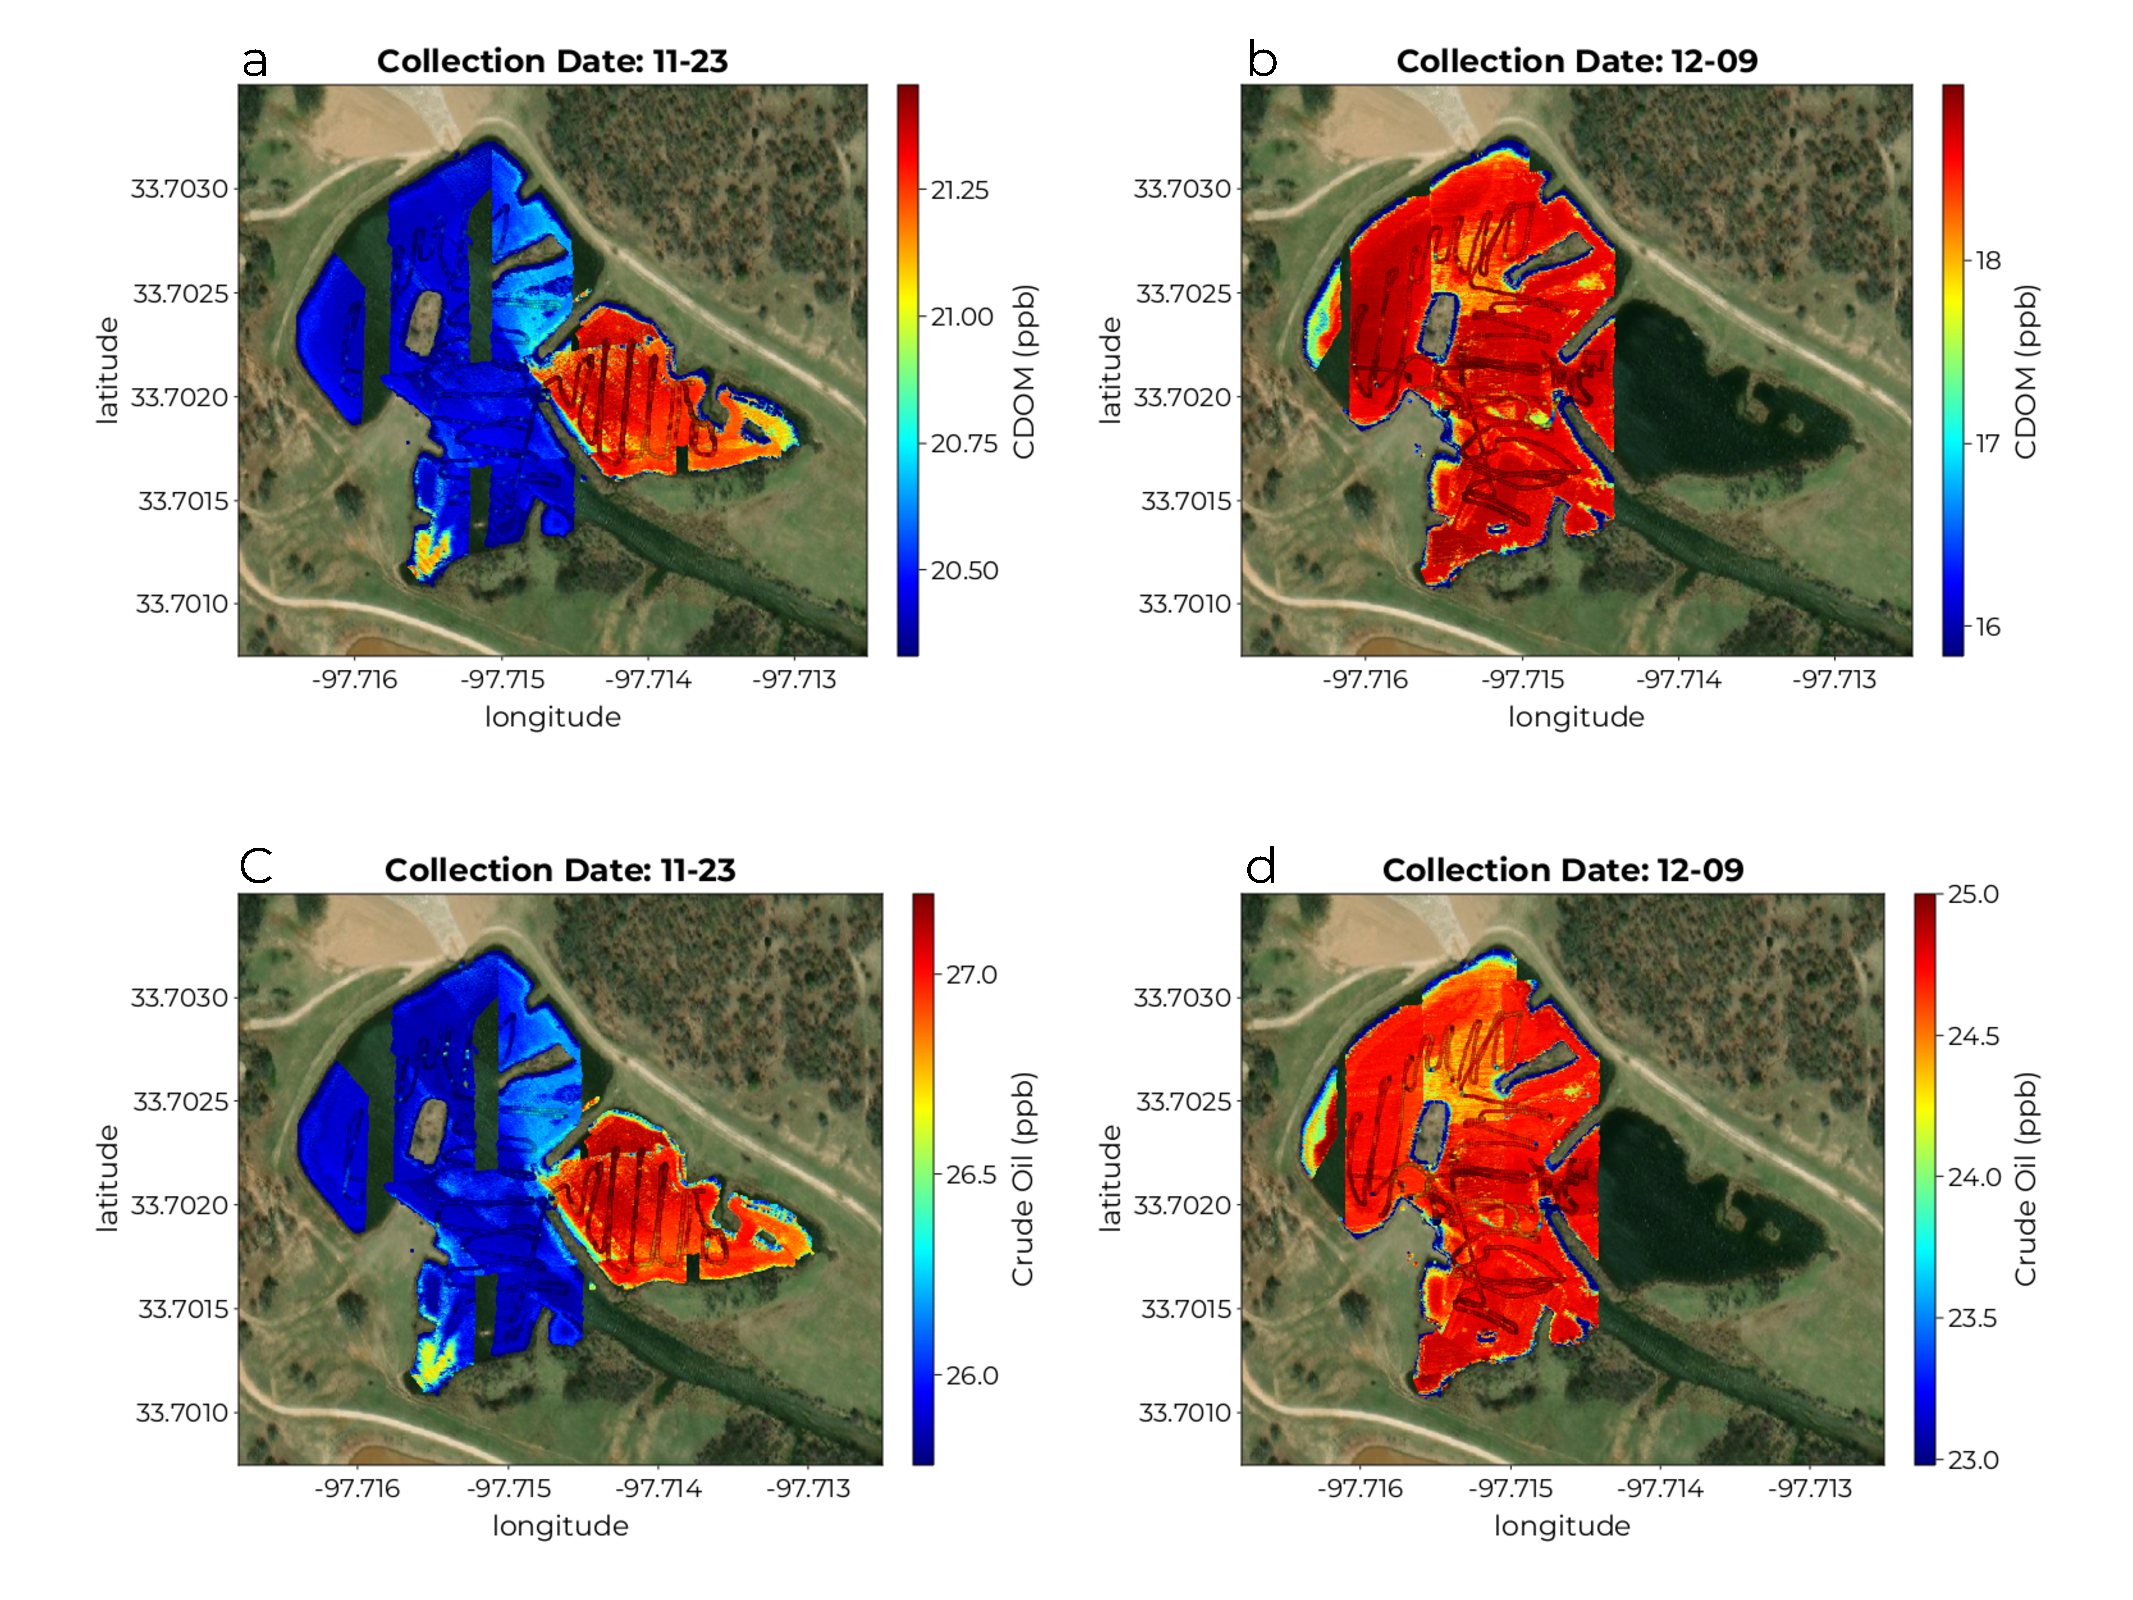
\includegraphics[width=18.0cm]{paper/figures/results/map-combined.pdf}
\end{adjustwidth}
\caption{Maps generated by applying the ML model to hyperspectral data cubes. (\textbf{a}) The CDOM model applied to the 11-23 collection. (\textbf{b}) The CDOM model applied the the 12-09 collection. (\textbf{c}) the Crude Oil model applied to the 11-23 collection. (\textbf{d}) The Crude Oil model applied to the 12-09 collection. In each panel, boat data are overlaid as color-filled squares. We note that there is good agreement between estimated values at boat locations and the in-situ reference measurements. \label{fig:maps}}
\end{figure}  


%%%%%%%%%%%%%%%%%%%%%%%%%%%%%%%%%%%%%%%%%%
\section{Discussion} \label{sec:discussion}


\subsection{Optically Active Components and Physio-Chemical Parameter Estimation}

We can probably explain the inference of salinity, ion concentrations, etc as being directly related to the observed concentrations of chlorophyll, cdom, co, bgm, etc... which are all optically active (i.e. have absorption features spectral region of our hyperspectral imager).

\begin{figure}[H]
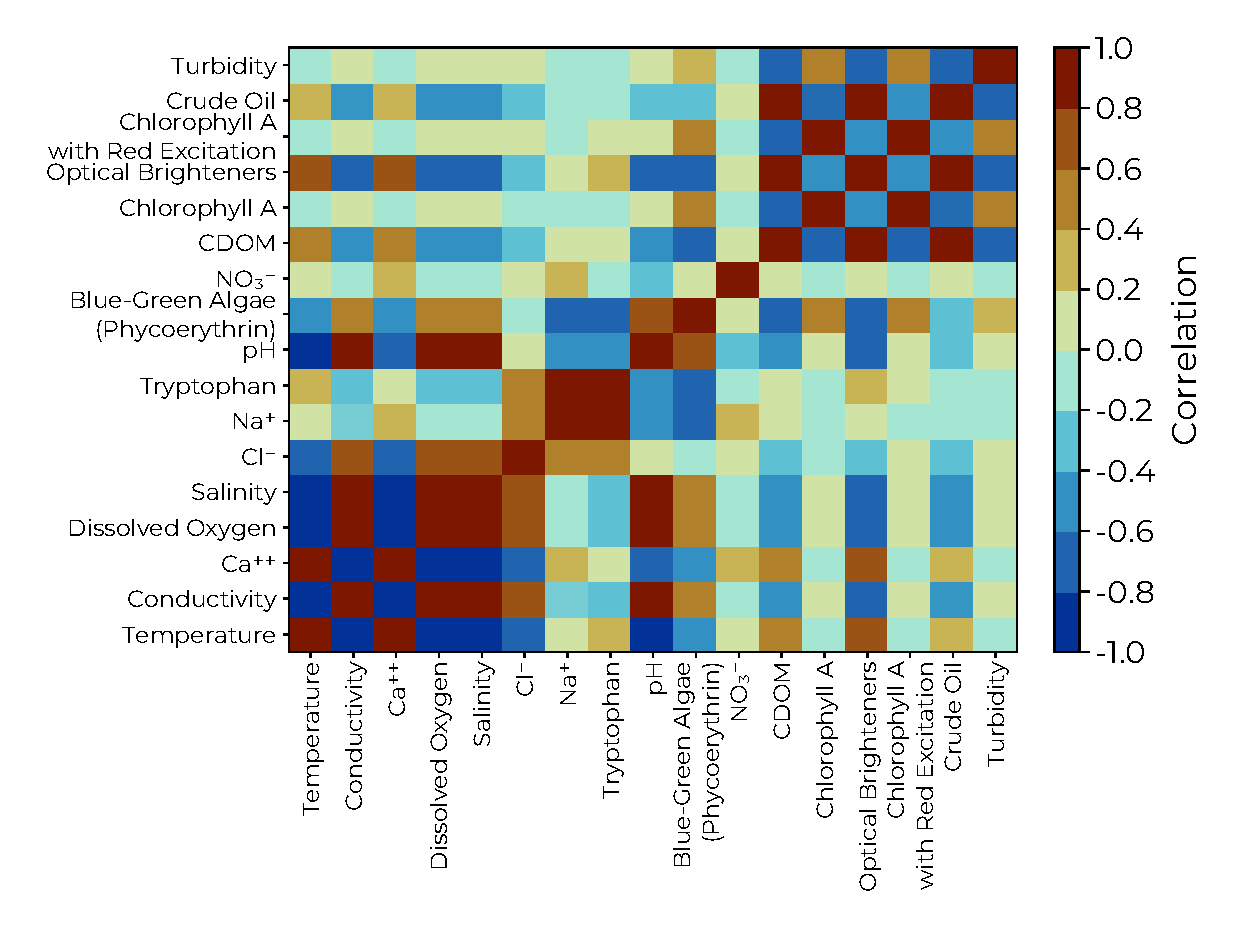
\includegraphics[width=10.5 cm]{paper/figures/results/target_correlations.pdf}
\caption{\label{fig:target-correlations}}
\end{figure}   



\subsection{Data Product Streaming}

\subsection{Limitations}

\begin{figure}[H]
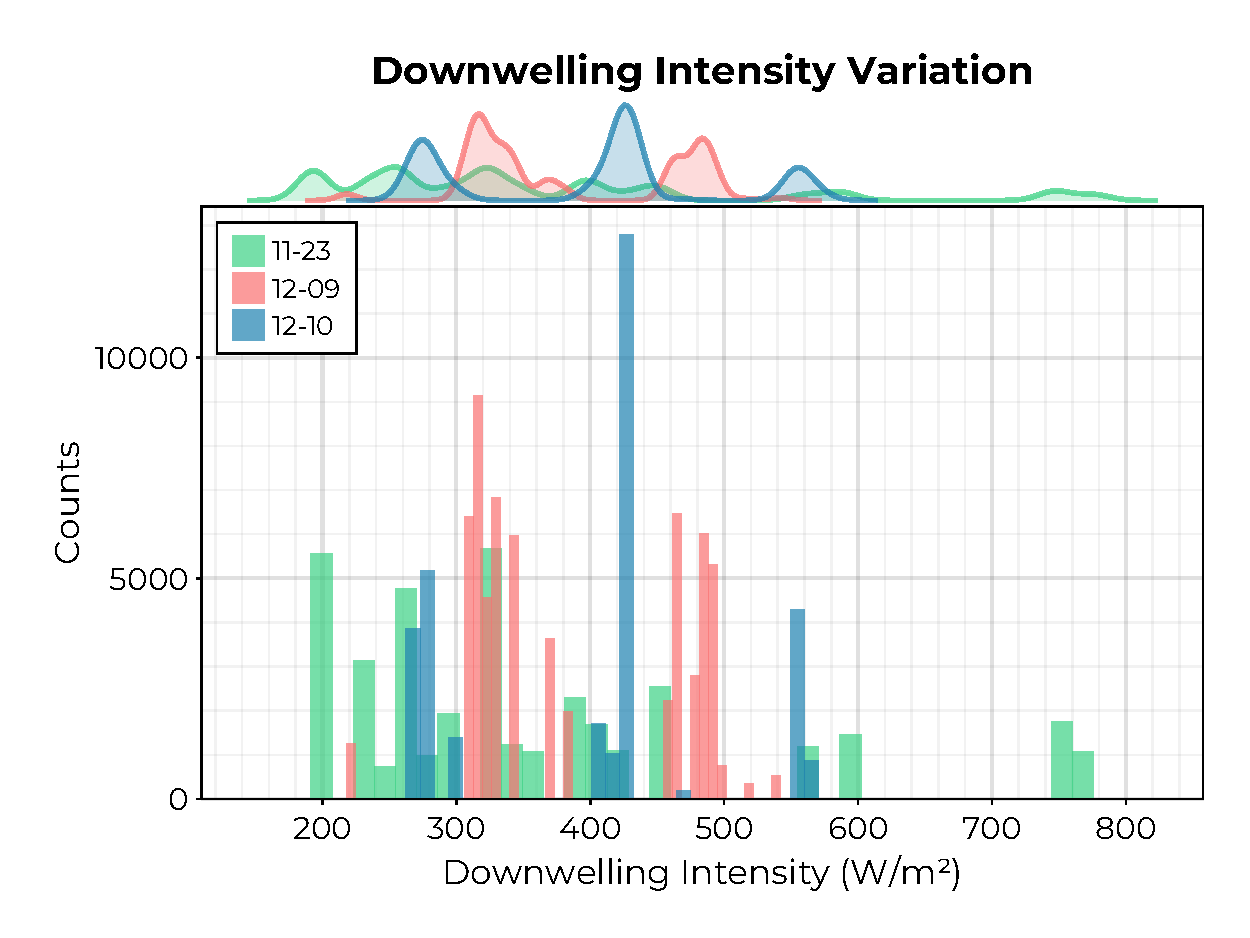
\includegraphics[width=10.5 cm]{paper/figures/results/downwelling-hist.pdf}
\caption{Distribution of total downwelling intensity during each of the three HSI collection flights. The multi-modal nature of these distributions reflects the impact of the relative orientation of the drone to the sun as well as potential occlusion due to the presence of clouds.\label{fig:downwelling-hist}}
\end{figure}   


\subsection{Extensions and Next Steps}

The current implementation of conformal prediction utilized in these models estimates a fixed width confidence interval for all outputs. This could be improved by training a secondary \textit{residual} model on the errors produced by the base learner, that is, a model which predicts 
\begin{equation}
    r(X) = \lvert f(X) - y \rvert = \lvert \hat{y} - y \rvert.
\end{equation}
In the conformal prediction framework, such a model could then be used to produce \textit{adaptive} uncertainty estimates using the augmented heuristic function
\begin{equation}
    S(X,y)  = \dfrac{\lvert \hat{y} - y \rvert }{r(X)}
\end{equation}
to produce scores on the calibration holdout set. With access to adaptive uncertainty estimates, we can then augment the navigation control for the USV to encourage data collection in regions of high model uncertainty. This would further optimize the data collection and calibration procedure at the expense of increased model training times. 



%%%%%%%%%%%%%%%%%%%%%%%%%%%%%%%%%%%%%%%%%%
\section{Conclusions}

This section is not mandatory, but can be added to the manuscript if the discussion is unusually long or complex.


%%%%%%%%%%%%%%%%%%%%%%%%%%%%%%%%%%%%%%%%%%
\vspace{6pt} 

%%%%%%%%%%%%%%%%%%%%%%%%%%%%%%%%%%%%%%%%%%
%% optional
\supplementary{The following supporting information can be downloaded at:  \linksupplementary{s1}, Table S1: Hyperspectral Reflectance Indices.}

% Only for journal Methods and Protocols:
% If you wish to submit a video article, please do so with any other supplementary material.
% \supplementary{The following supporting information can be downloaded at: \linksupplementary{s1}, Figure S1: title; Table S1: title; Video S1: title. A supporting video article is available at doi: link.}

% Only for journal Hardware:
% If you wish to submit a video article, please do so with any other supplementary material.
% \supplementary{The following supporting information can be downloaded at: \linksupplementary{s1}, Figure S1: title; Table S1: title; Video S1: title.\vspace{6pt}\\
%\begin{tabularx}{\textwidth}{lll}
%\toprule
%\textbf{Name} & \textbf{Type} & \textbf{Description} \\
%\midrule
%S1 & Python script (.py) & Script of python source code used in XX \\
%S2 & Text (.txt) & Script of modelling code used to make Figure X \\
%S3 & Text (.txt) & Raw data from experiment X \\
%S4 & Video (.mp4) & Video demonstrating the hardware in use \\
%... & ... & ... \\
%\bottomrule
%\end{tabularx}
%}

%%%%%%%%%%%%%%%%%%%%%%%%%%%%%%%%%%%%%%%%%%
\authorcontributions{For research articles with several authors, a short paragraph specifying their individual contributions must be provided. The following statements should be used ``Conceptualization, X.X. and Y.Y.; methodology, X.X.; software, X.X.; validation, X.X., Y.Y. and Z.Z.; formal analysis, X.X.; investigation, X.X.; resources, X.X.; data curation, X.X.; writing---original draft preparation, X.X.; writing---review and editing, X.X.; visualization, X.X.; supervision, X.X.; project administration, X.X.; funding acquisition, Y.Y. All authors have read and agreed to the published version of the manuscript.'', please turn to the  \href{http://img.mdpi.org/data/contributor-role-instruction.pdf}{CRediT taxonomy} for the term explanation. Authorship must be limited to those who have contributed substantially to the work~reported.}

\funding{Please add: ``This research received no external funding'' or ``This research was funded by NAME OF FUNDER grant number XXX.'' and  and ``The APC was funded by XXX''. Check carefully that the details given are accurate and use the standard spelling of funding agency names at \url{https://search.crossref.org/funding}, any errors may affect your future funding.}

\institutionalreview{Not applicable}

\informedconsent{Not applicable}

\dataavailability{We encourage all authors of articles published in MDPI journals to share their research data. In this section, please provide details regarding where data supporting reported results can be found, including links to publicly archived datasets analyzed or generated during the study. Where no new data were created, or where data is unavailable due to privacy or ethical restrictions, a statement is still required. Suggested Data Availability Statements are available in section ``MDPI Research Data Policies'' at \url{https://www.mdpi.com/ethics}.} 

% Only for journal Nursing Reports
%\publicinvolvement{Please describe how the public (patients, consumers, carers) were involved in the research. Consider reporting against the GRIPP2 (Guidance for Reporting Involvement of Patients and the Public) checklist. If the public were not involved in any aspect of the research add: ``No public involvement in any aspect of this research''.}

% Only for journal Nursing Reports
%\guidelinesstandards{Please add a statement indicating which reporting guideline was used when drafting the report. For example, ``This manuscript was drafted against the XXX (the full name of reporting guidelines and citation) for XXX (type of research) research''. A complete list of reporting guidelines can be accessed via the equator network: \url{https://www.equator-network.org/}.}

\acknowledgments{In this section you can acknowledge any support given which is not covered by the author contribution or funding sections. This may include administrative and technical support, or donations in kind (e.g., materials used for experiments).}

\conflictsofinterest{The authors declare no conflicts of interest.}

%%%%%%%%%%%%%%%%%%%%%%%%%%%%%%%%%%%%%%%%%%
%% Optional

%% Only for journal Encyclopedia
%\entrylink{The Link to this entry published on the encyclopedia platform.}

\abbreviations{Abbreviations}{
The following abbreviations are used in this manuscript:\\

\noindent 
\begin{tabular}{@{}ll}
MDPI & Multidisciplinary Digital Publishing Institute\\
DOAJ & Directory of open access journals\\
TLA & Three letter acronym\\
LD & Linear dichroism
\end{tabular}
}

%%%%%%%%%%%%%%%%%%%%%%%%%%%%%%%%%%%%%%%%%%
%% Optional
\appendixtitles{no} % Leave argument "no" if all appendix headings stay EMPTY (then no dot is printed after "Appendix A"). If the appendix sections contain a heading then change the argument to "yes".
\appendixstart
\appendix
%% \section[\appendixname~\thesection]{}\label{appendix:spec-indices}
%% \subsection[\appendixname~\thesubsection]{}


%%%%%%%%%%%%%%%%%%%%%%%%%%%%%%%%%%%%%%%%%%
\begin{adjustwidth}{-\extralength}{0cm}
%\printendnotes[custom] % Un-comment to print a list of endnotes

\reftitle{References}

% Please provide either the correct journal abbreviation (e.g. according to the “List of Title Word Abbreviations” http://www.issn.org/services/online-services/access-to-the-ltwa/) or the full name of the journal.
% Citations and References in Supplementary files are permitted provided that they also appear in the reference list here. 

%=====================================
% References, variant A: external bibliography
%=====================================

\bibliography{references.bib}


% If authors have biography, please use the format below
%\section*{Short Biography of Authors}
%\bio
%{\raisebox{-0.35cm}{\includegraphics[width=3.5cm,height=5.3cm,clip,keepaspectratio]{Definitions/author1.pdf}}}
%{\textbf{Firstname Lastname} Biography of first author}
%
%\bio
%{\raisebox{-0.35cm}{\includegraphics[width=3.5cm,height=5.3cm,clip,keepaspectratio]{Definitions/author2.jpg}}}
%{\textbf{Firstname Lastname} Biography of second author}

% For the MDPI journals use author-date citation, please follow the formatting guidelines on http://www.mdpi.com/authors/references
% To cite two works by the same author: \citeauthor{ref-journal-1a} (\citeyear{ref-journal-1a}, \citeyear{ref-journal-1b}). This produces: Whittaker (1967, 1975)
% To cite two works by the same author with specific pages: \citeauthor{ref-journal-3a} (\citeyear{ref-journal-3a}, p. 328; \citeyear{ref-journal-3b}, p.475). This produces: Wong (1999, p. 328; 2000, p. 475)

%%%%%%%%%%%%%%%%%%%%%%%%%%%%%%%%%%%%%%%%%%
%% for journal Sci
%\reviewreports{\\
%Reviewer 1 comments and authors’ response\\
%Reviewer 2 comments and authors’ response\\
%Reviewer 3 comments and authors’ response
%}
%%%%%%%%%%%%%%%%%%%%%%%%%%%%%%%%%%%%%%%%%%
\PublishersNote{}
\end{adjustwidth}
\end{document}
